\documentclass[
	fontsize=11pt,
	paper=a4,
	foldmarks=false
]{scrartcl}

\usepackage{adjustbox}
\usepackage{algorithm}
\usepackage{algpseudocode}
\usepackage{amsfonts}
\usepackage{amsmath}
\usepackage{amssymb}
\usepackage{amsthm}
\usepackage{booktabs}
\usepackage{cases}
\usepackage{cite}
\usepackage[acronym]{glossaries-extra}
\usepackage{hyperref}
\usepackage{mathtools}
\usepackage[nopatch=footnote]{microtype}
\usepackage[short]{optidef}
\usepackage{pgfplots}
\usepackage[subtle]{savetrees}
\usepackage{siunitx}
\usepackage[caption=false,font=footnotesize,subrefformat=parens,labelformat=parens]{subfig}
\usepackage{tabularx}
\usepackage{tikz}
\usepackage{epstopdf}
\usepackage{multirow}
\usepackage{enumitem}

% amsmath
\allowdisplaybreaks
\DeclareMathOperator{\diag}{diag}
\DeclareMathOperator{\tr}{tr}
\DeclareMathOperator{\sv}{sv}
% \DeclareMathOperator{\card}{card}
\DeclareMathOperator{\conv}{conv}
\DeclareMathOperator{\rank}{rank}
\DeclareMathOperator{\ran}{ran}
% \DeclareMathOperator{\ker}{ker}

% amsthm
\theoremstyle{plain}
\newtheorem{proposition}{Proposition}
\newtheorem{corollary}{Corollary}[proposition]
\newtheorem{lemma}{Lemma}

\theoremstyle{definition}
\newtheorem{definition}{Definition}
\newtheorem{example}{Example}
\newtheorem{remark}{Remark}

% enumitem
\setlist[itemize]{leftmargin=5mm}
\setlist[enumerate]{leftmargin=5mm}

% PGF/TikZ
\usetikzlibrary{arrows,calc,matrix,patterns,plotmarks,positioning,shapes}
\usetikzlibrary{decorations.pathmorphing,decorations.pathreplacing,decorations.shapes,shapes.geometric}
\usepgfplotslibrary{groupplots,patchplots}
\pgfplotsset{compat=1.18}
\pgfplotsset{every axis/.append style={
			title style={font=\Large},
			label style={font=\Large},
			tick label style={font=\Large},
			legend style={font=\large},
		}}

% algorithmicx
\algrenewcommand{\algorithmicrequire}{\textbf{Input:}}
\algrenewcommand{\algorithmicensure}{\textbf{Output:}}
\algrenewcommand{\algorithmicwhile}{\textbf{While}}
\algrenewcommand{\algorithmicend}{\textbf{End}}
\algrenewcommand{\algorithmicrepeat}{\textbf{Repeat}}
\algrenewcommand{\algorithmicuntil}{\textbf{Until}}
\algrenewcommand{\algorithmicfor}{\textbf{For}}
\algrenewcommand{\algorithmicif}{\textbf{If}}
\algrenewcommand{\algorithmicelse}{\textbf{Else}}
\algrenewcommand{\algorithmicdo}{}
\algrenewcommand{\algorithmicthen}{}
\algnewcommand{\Initialize}[1]{%
	\State \textbf{Initialize }{#1}
}

% glossaries-extra
\glsdisablehyper
\setabbreviationstyle[acronym]{long-short}
\newacronym{ao}{AO}{Alternating Optimization}
\newacronym{bd}{BD}{Beyond Diagonal}
\newacronym{bcd}{BCD}{Block Coordinate Descent}
\newacronym{d}{D}{Diagonal}
\newacronym{dof}{DoF}{Degrees of Freedom}
\newacronym{siso}{SISO}{Single-Input Single-Output}
\newacronym{miso}{MISO}{Multiple-Input Single-Output}
\newacronym{mimo}{MIMO}{Multiple-Input Multiple-Output}
\newacronym{rcg}{RCG}{Riemannian Conjugate Gradient}
\newacronym{ris}{RIS}{Reconfigurable Intelligent Surface}
\newacronym{gp}{GP}{Globally Passive}
\newacronym{pc}{PC}{Point-to-Point Channel}
\newacronym{p2p}{P2P}{Point-to-Point}
\newacronym{ic}{IC}{Interference Channel}
\newacronym{qos}{QoS}{Quality of Service}
\newacronym{wsr}{WSR}{Weighted Sum-Rate}
\newacronym{snr}{SNR}{Signal-to-Noise Ratio}
\newacronym{svd}{SVD}{Singular Value Decomposition}
\newacronym{mmse}{MMSE}{Minimum Mean-Square Error}
\newacronym{wmmse}{WMMSE}{Weighted \gls{mmse}}
\newacronym{mse}{MSE}{Mean-Square Error}
\newacronym{los}{LoS}{Line-of-Sight}
\newacronym{csi}{CSI}{Channel State Information}
\newacronym{cscg}{CSCG}{Circularly Symmetric Complex Gaussian}
\newacronym{sca}{SCA}{Successive Convex Approximation}
\newacronym{kkt}{KKT}{Karush-Kuhn-Tucker}
\newacronym{rf}{RF}{Radio Frequency}

% * page limit hacks
% \captionsetup[subfloat]{farskip=1pt,captionskip=1pt}
% \setlength{\abovecaptionskip}{0pt plus 0pt minus 0pt}

% \setlist{nosep}

% \usepackage{xpatch}
% \setlength{\topsep}{0pt}
% \setlength{\partopsep}{0pt plus 0pt minus 0pt}
% \setlength{\parskip}{0pt}
% \setlength{\parindent}{0pt}
% \makeatletter
% \def\thm@space@setup{%
% 	\thm@preskip=1mm
% 	\thm@postskip=\thm@preskip % or whatever, if you don't want them to be equal
% }
% \xpatchcmd{\proof}{\topsep6\p@\@plus6\p@\relax}{}{}{}
% \makeatother

% \usepackage{titlesec}
% \def\subparagraph{}
% \titlespacing*{\section}{0pt}{0pt}{0pt}
% \titlespacing{\subsection}{0pt}{0pt}{0pt}
% \renewcommand{\thesubsubsection}{\arabic{subsubsection}}
% \titleformat{\subsubsection}[runin]{\itshape}{\thesubsubsection)}{1ex}{}
% \titlespacing*{\subsubsection}{0pt}{0pt}{*1}

% \usepackage{setspace}
% \abovedisplayskip=1mm
% \belowdisplayskip=1mm
% \abovedisplayshortskip=1mm
% \belowdisplayshortskip=1mm
% \setlength{\jot}{0.1mm}
% \setlength{\floatsep}{1mm}
% \setlength{\textfloatsep}{1mm}
% \setlength{\intextsep}{1mm}
% \setlength{\skip\footins}{1mm}
% \addtolength{\parindent}{-1mm}

% * legacy
% % Double superscript
% \newcommand\herm[2][-4]{{#2}^{\mkern#1mu\mathsf{H}}}

% % algpseudocode
% \makeatletter
% \renewcommand{\fnum@algorithm}{\fname@algorithm{} \thealgorithm:}
% \newcommand\setalgorithmcaptionfont[1]{%
% 	\let\my@floatc@ruled\floatc@ruled          % save \floatc@ruled
% 	\def\floatc@ruled{%
% 		\global\let\floatc@ruled\my@floatc@ruled % restore \floatc@ruled
% 		#1\floatc@ruled}}
% \makeatother

\usepackage{response}


\setkomavar{signature}{Yang Zhao, Hongyu Li, Bruno Clerckx, and Massimo Franceschetti}
\setkomavar{date}{\today}
\setkomavar{subject}{Response to Decision on Manuscript T-SP-32387-2024}

\begin{document}
\begin{letter}{%
		Prof. Wei Yi\\
		Associate Editor\\
		IEEE Transactions on Signal Processing
	}
	\opening{Dear Editor and Reviewers,}
	Thank you for giving us the opportunity to submit a revised version of T-SP-32387-2024.
	Your comments and suggestions have been invaluable in helping us improve the quality of the manuscript.
	Below we prepare a point-to-point response and highlight the corresponding in-text changes, where labels have been matched to the latest version for your convenience.
	The title has been changed to \emph{MIMO Channel Shaping and Rate Maximization Using Beyond Diagonal RIS} to better reflect the content of the manuscript.
	We hope that the revisions and clarifications make the manuscript meet the standards of TSP publications.
	\closing{Yours sincerely,}
\end{letter}


\begin{editor}
	\summary{
		The reviewers raised a number of concerns regarding the paper's contribution, novelty, and mathematical correctness, which led to the recommendation for rejection. The main issues identified include:
		\begin{enumerate}
			\item The contribution of the paper is unclear. Specifically, the proposed framework in \eqref{op:shaping} is not sufficiently general as it does not consider \gls{bd}-\gls{ris} dependent constraints (e.g., \gls{qos}, sensing quality). A more general case has already been investigated and solved in the authors' previous work \cite{Zhou2023}. Some content in Section \ref{sc:shaping_numerical} are well established methods in the literature \cite{Abrudan2008}.
			\item The optimization problems \eqref{op:power} and \eqref{op:rate_ris} lacks of novelty. The reviewer pointed that they can be possibly solved by existing methods through appropriate adjustment \cite{Santamaria2023,Li2023b}. Also, it is also pointed out that Corollaries \ref{co:nd_sv_prod_subset} -- \ref{co:nd_sv_prod_tail} are the standard results from matrix textbook.
			\item The correctness and usefulness of the mathematical derivations. For example, the derivation in the proof of Appendix \ref{ap:shaping} is incorrect. Convergence proof in Appendix \ref{ap:power} is questionable. The usefulness of these bounds on singular values of the effective channel $\mathbf{H}$ is unclear.
			\item The literature review can be enhanced to cover a boarder range of papers that related to the problem addressed.
			\item The simulation study can be enhanced. For example, comparisons with the \gls{d}-\gls{ris} and a globally passive \gls{bd}-\gls{ris} were suggested by the reviewer.
		\end{enumerate}
	}

	\reply{
		We appreciate the editor's summary of the comments. We have carefully considered each point raised and have made significant revisions to address these concerns. Please refer to the following responses for a detailed explanation of the changes made in the revised manuscript.
	}

\end{editor}

\begin{reviewer}
	\summary{
		This manuscript investigates the impact of \gls{bd}-\gls{ris} to the distribution of singular values of \gls{mimo} channel of a point-to-point communication system. Especially, the authors derive bounds of singular values of \gls{bd}-\gls{ris} channel and propose algorithms to design \gls{bd}-\gls{ris} configuration.
	}

	\comment{
		The contribution of Sec. \ref{sc:shaping_numerical} is unclear for the following two reasons.
		\begin{enumerate}
			\item The manuscript claims to propose a universal optimization framework for \gls{bd}-\gls{ris} as in \eqref{op:shaping}. However, the framework in \eqref{op:shaping} is indeed not sufficiently general. It does not consider \gls{bd}-\gls{ris} dependent constraints (e.g., \gls{qos}, sensing quality) besides the orthogonal conditions \eqref{cn:shaping_unitary}. The reviewer notice that a more general framework, which considers \gls{bd}-\gls{ris} constraints in addition to \eqref{cn:shaping_unitary}, has already been investigated and solved in the authors' previous work \cite{Zhou2023}.
			\item Besides, both the non-geodesic \gls{rcg} and geodesic \gls{rcg} algorithms, e.g., \eqref{eq:gradient_eucl} -- \eqref{eq:geodesic_tran}, are well established methods in the literature, e.g., \cite{Abrudan2008}. Therefore, the novelty of Sec. \ref{sc:shaping_numerical} unclear.
		\end{enumerate}
	}

	\reply{
		We appreciate the reviewer's insightful comments.
		The claim of ``universal optimization framework'' and the non-geodesic \gls{rcg} method have been removed from the revised manuscript, and we have carefully rephrased Sections \ref{sc:contributions} and \ref{sc:shaping_numerical} to reflect the specific contributions of our work.
		Indeed, the geodesic \gls{rcg} algorithm is well studied in the literature and our intention was to extend it to block-unitary cases with parallel or unified updates, which is particularly suitable for the design of group-connected \gls{bd}-\gls{ris}.
	}

	\comment{
		In Sec. \ref{sc:shaping_numerical}, the manuscript proposes to maximize weighted sum of singular values of the effective channel $\mathbf{H}$. The optimization objective is rather vague. Is the weighted sum of singular values related to any meaningful performance metric (e.g., capacity, power gain, and so on)?
	}

	\reply{
		We agree with the reviewer that the optimization objective of weighted sum of singular values is not directly related to a specific performance metric.
		However, it helps to reveal the achievable region of channel singular values (which covers all related metrics) and we believe itself could serve as a metric for measuring the \gls{mimo} channel shaping capability of different \gls{ris}.
		In the revised manuscript, we also generalize the objective to symmetric gauge functions to further address this concern.

		\change{
			Consider a special class of channel shaping problem
			\begin{maxi*}
				{\scriptstyle{\mathbf{\Theta}}}{f\bigl(\sv(\mathbf{H})\bigr)}{}{}
				\addConstraint{\mathbf{\Theta}_g^\mathsf{H} \mathbf{\Theta}_g=\mathbf{I},}{\quad \forall g,}{}
			\end{maxi*}
			where $f: \mathbb{R}^{N} \to \mathbb{R}$ is a symmetric gauge function (i.e., a norm invariant under sign change and argument permutation) \cite{Watson1992}.
			Examples of such $f$ include the Ky Fan $k$ norm, Schatten $p$ norm, $n$-th singular value, and channel power gain.
		}
	}

	\comment{
		Derivation in the proof of Appendix \ref{ap:shaping} is incorrect. Specifically, $(\partial \mathbf{u}^\mathsf{T}) \cdot \mathbf{u}$ is not equal to $\partial (\mathbf{u}^T \mathbf{u})$. Similar error occurs to $\mathbf{v}$. Please note that the derivative of singular value of a matrix with respect to the matrix itself does not exist. In fact, sub-differential should be used instead, e.g., \cite{Cai2010}.
	}

	\reply{
		We appreciate the reviewer's careful reading of the manuscript.
		We have corrected the derivation in the proof of Appendix \ref{ap:shaping} and have used the sub-differential to handle the non-differentiability of the singular value function.
		\change{
			\setcounter{proposition}{3}
			\begin{proposition}
				The sub-differential of \eqref{ob:shaping} with respect to \gls{bd}-\gls{ris} block $g$ is
				\begin{equation*}
					\partial_{\mathbf{\Theta}_g^*} f\bigl(\sv(\mathbf{H})\bigr) = \conv \bigl\{ \mathbf{H}_{\mathrm{B},g}^\mathsf{H} \mathbf{U} \mathbf{D} \mathbf{V}^\mathsf{H} \mathbf{H}_{\mathrm{F},g}^\mathsf{H} \bigr\},
				\end{equation*}
				where $\mathbf{D} \in \mathbb{C}^{N_\mathrm{R} \times N_\mathrm{T}}$ is a rectangular diagonal matrix with $[\mathbf{D}]_{n,n} \in \partial_{\sigma_n(\mathbf{H})} f\bigl(\sv(\mathbf{H})\bigr)$, $\forall n \in [N]$, and $\mathbf{U}$, $\mathbf{V}$ are any left and right singular matrices of $\mathbf{H}$.
			\end{proposition}
		}
	}

	\comment{
		The rank equation in the proof of Prop. \ref{pp:dof} (Appendix \ref{ap:dof}) seems confusing. The rank of product of two matrices is: $\rank(\mathbf{AB}) = \rank(\mathbf{B}) - \dim(\ker(\mathbf{A}) \cap \ran(\mathbf{B}))$. How could one obtain the rank equation in Appendix \ref{ap:dof}? Please clarify.
	}

	\reply{
		Using the rank equation pointed out by the reviewer, we realized that the achievability proof in the previous version was incorrect. In fact, the proposition was incorrect.
		A new proof in Appendix \ref{ap:dof} shows that \gls{bd}-\gls{ris} may achieve a larger or smaller number of \gls{mimo} \gls{dof} than \gls{d}-\gls{ris}.
		We apologize for the confusion and appreciate the reviewer for pointing out this mistake.
		\change{
			\setcounter{proposition}{0}
			\begin{proposition}[Degrees of freedom]
				\gls{bd}-\gls{ris} may achieve a larger or smaller number of \gls{mimo} \gls{dof} than \gls{d}-\gls{ris}.
			\end{proposition}
		}
	}

	\comment{
		In Sec. \ref{sc:shaping_analytical}, the manuscript provides a number of bounds on singular values of the effective channel $\mathbf{H}$. However, the usefulness of these bounds is unclear. What can these bounds be used for? Note the results in Corollaries \ref{co:nd_sv_prod_subset} -- \ref{co:nd_sv_prod_tail} are quite standard results from matrix textbook. The (upper) bound in Corollary \ref{co:nd_power}, which is achieved by aligning its left and right singular-value vectors to that of the forward and backward channels, respectively, is reminiscent of the results in seminal papers on relay beamforming design, e.g., \cite{Rong2009,Rong2009a}.
	}

	\reply{
		The aim of Proposition \ref{pp:nd} is to transform the channel shaping limit question into a well-studied linear algebra question, such that Corollaries \ref{co:nd_sv_prod_subset} -- \ref{co:nd_sv_prod_tail} (previously 3.1 -- 3.4) follows from standard results.
		In the revised manuscript, we have also added
		\begin{itemize}
			\item Upper and lower bounds on individual singular value in Corollary \ref{co:nd_sv_indl};
			\item Lower bound on channel power gain in Corollary \ref{co:nd_power};
			\item Upper bound on channel capacity at general and extreme \gls{snr} in Corollaries \ref{co:nd_capacity_snr_general} and \ref{co:nd_capacity_snr_extreme};
		\end{itemize}
		and derived the corresponding \gls{ris} scattering matrices in closed form.
		We also notice that the bounds on the $n$-th singular value can be used, for example, to simplify the precoder design in \gls{mimo} systems with limited number $n$ of RF chains.
		The comparison to relay beamforming design is insightful and we have added footnote \ref{fn:power_nd_max} to highlight the connection.
		\change{
			\setcounter{proposition}{3}
			\setcounter{corollary}{2}
			\begin{corollary}[Individual singular value]
				If the direct channel is negligible,
				then the $n$-th channel singular value can be manipulated up to
				\begin{equation*}
					\max_{\mathclap{i+j=n+N_\mathrm{S}}} \ \sigma_i(\mathbf{H}_\mathrm{B}) \sigma_j(\mathbf{H}_\mathrm{F}) \le \sigma_n(\mathbf{H}) \le \min_{\mathclap{i+j=n+1}} \ \sigma_i(\mathbf{H}_\mathrm{B}) \sigma_j(\mathbf{H}_\mathrm{F}),
				\end{equation*}
				where $(i, j) \in [N_\mathrm{S}]^2$.
				The upper and lower bounds are attained respectively at
				\begin{align*}
					\mathbf{\Theta}_{\textnormal{sv-}n\textnormal{-max}}^\textnormal{MIMO-ND} & = \mathbf{V}_\mathrm{B} \mathbf{P} \mathbf{U}_\mathrm{F}^\mathsf{H}, \\
					\mathbf{\Theta}_{\textnormal{sv-}n\textnormal{-min}}^\textnormal{MIMO-ND} & = \mathbf{V}_\mathrm{B} \mathbf{Q} \mathbf{U}_\mathrm{F}^\mathsf{H},
				\end{align*}
				where $\mathbf{V}_\mathrm{B}, \mathbf{U}_\mathrm{F} \in \mathbb{U}^{N_\mathrm{S} \times N_\mathrm{S}}$ are any right and left singular matrices\footnotetext{%
					We highlight the non-uniqueness of $\mathbf{V}_\mathrm{B}$ and $\mathbf{U}_\mathrm{F}$. When a singular value has multiplicity $k$, the corresponding singular vectors can be any orthonormal basis of the $k$-dimensional subspace. Even if all singular values are distinct, the singular vectors of each can be scaled by a phase factor of choice.} of $\mathbf{H}_\mathrm{B}$ and $\mathbf{H}_\mathrm{F}$, respectively,
				and $\mathbf{P}$ and $\mathbf{Q}$ are arbitrary permutation matrices of dimension $N_\mathrm{S}$ satisfying:
				\begin{itemize}
					\item The $(i, j)$-th entry is $1$, where
					\begin{align*}
						(i, j) &=
						\begin{cases}
							\underset{\mathclap{i+j=n+1}}{\arg\min} \ \sigma_i(\mathbf{H}_\mathrm{B}) \sigma_j(\mathbf{H}_\mathrm{F}), & \text{for } \mathbf{P}, \\
							\underset{\mathclap{i+j=n+N_\mathrm{S}}}{\arg\max} \ \sigma_i(\mathbf{H}_\mathrm{B}) \sigma_j(\mathbf{H}_\mathrm{F}), & \text{for } \mathbf{Q}.
						\end{cases}
					\end{align*}
					and ties may be broken arbitrarily;
					\item After deleting the $i$-th row and $j$-th column, the resulting submatrix $\mathbf{Y}$ is arbitrary permutation matrix of dimension $N_\mathrm{S}-1$ satisfying
					\begin{alignat*}{2}
						\sigma_{n{-}1}(\hat{\mathbf{\Sigma}}_{\mathrm{B}} \mathbf{Y} \hat{\mathbf{\Sigma}}_{\mathrm{F}}) & {\ge} \ \ \min_{\mathclap{i+j=n+1}} \ \sigma_i(\mathbf{H}_\mathrm{B}) \sigma_j(\mathbf{H}_\mathrm{F})            &  & \text{ for } \mathbf{P}, \\
						\sigma_{n{+}1}(\hat{\mathbf{\Sigma}}_{\mathrm{B}} \mathbf{Y} \hat{\mathbf{\Sigma}}_{\mathrm{F}}) & {\le} \ \ \max_{\mathclap{i+j=n+N_\mathrm{S}}} \ \sigma_i(\mathbf{H}_\mathrm{B}) \sigma_j(\mathbf{H}_\mathrm{F}) &  & \text{ for } \mathbf{Q},
					\end{alignat*}
					where $\hat{\mathbf{\Sigma}}_{\mathrm{B}}$ and $\hat{\mathbf{\Sigma}}_{\mathrm{F}}$ are diagonal singular value matrices of $\mathbf{H}_\mathrm{B}$ and $\mathbf{H}_\mathrm{F}$ with both $i$-th row and $j$-th column deleted, respectively.
				\end{itemize}
			\end{corollary}
		}

		\change{
			\begin{corollary}[Channel power gain]
				If the direct channel is negligible, then the channel power gain is bounded from above (resp. below) by the inner product of squared singular values of $\mathbf{H}_\mathrm{B}$ and $\mathbf{H}_\mathrm{F}$ when they are sorted similarly (resp. oppositely), that is,\footnotetext{As a side note, we notice \cite{Fang1994} discussed a similar bound using extreme singular values $\max\bigl(\sigma_{N}(\mathbf{H}_\mathrm{B}) \lVert \mathbf{H}_\mathrm{F} \rVert _\mathrm{F}^2, \sigma_{N}(\mathbf{H}_\mathrm{F}) \lVert \mathbf{H}_\mathrm{B} \rVert _\mathrm{F}^2\bigr) \le \lVert \mathbf{H} \rVert _\mathrm{F}^2 \le \min\bigl(\sigma_1(\mathbf{H}_\mathrm{B}) \lVert \mathbf{H}_\mathrm{F} \rVert _\mathrm{F}^2, \sigma_1(\mathbf{H}_\mathrm{F}) \lVert \mathbf{H}_\mathrm{B} \rVert _\mathrm{F}^2\bigr)$. This is a looser version of \eqref{iq:power_nd} and cannot take equalities unless the extreme singular values are of multiplicity $N$.}
				\begin{equation*}
					\sum_{n=1}^N \sigma_n^2(\mathbf{H}_\mathrm{B}) \sigma_{N_\mathrm{S}-n+1}^2(\mathbf{H}_\mathrm{F}) \le \lVert \mathbf{H} \rVert _\mathrm{F}^2 \le \sum_{n=1}^N \sigma_n^2(\mathbf{H}_\mathrm{B}) \sigma_n^2(\mathbf{H}_\mathrm{F}),
				\end{equation*}
				whose upper\footnotetext{The upper bound \eqref{eq:ris_nd_power_max} is reminiscent of the optimal amplify-and-forward relay beamforming design \cite[(16), (17)]{Rong2009a} where the diagonal matrices boil down to $\mathbf{I}$ due to the passive nature of \gls{ris}.} and lower bounds are attained respectively at
				\begin{align*}
					\mathbf{\Theta}_\textnormal{P-max}^\textnormal{MIMO-ND} & = \mathbf{V}_\mathrm{B} \mathbf{U}_\mathrm{F}^\mathsf{H},             \\
					\mathbf{\Theta}_\textnormal{P-min}^\textnormal{MIMO-ND} & = \mathbf{V}_\mathrm{B} \mathbf{J} \mathbf{U}_\mathrm{F}^\mathsf{H},
				\end{align*}
				where $\mathbf{J}$ is the exchange (a.k.a. backward identity) matrix of dimension $N_\mathrm{S}$.
			\end{corollary}
		}

		\change{
			\begin{corollary}[Channel capacity at general \gls{snr}]
				If the direct channel is negligible, then the \gls{bd}-\gls{ris} aided \gls{mimo} channel capacity is
				\begin{equation*}
					C^\textnormal{MIMO-ND} = \sum_{n=1}^N \log \left(1 + \frac{s_n \sigma_n^2(\mathbf{H}_\mathrm{B}) \sigma_n^2(\mathbf{H}_\mathrm{F})}{\eta}\right),
				\end{equation*}
				where $\eta$ is the average noise power, $s_n = \mu - \frac{\eta}{\sigma_n^2(\mathbf{H}_\mathrm{B}) \sigma_n^2(\mathbf{H}_\mathrm{F})}$ is the power allocated to the $n$-th mode obtainable by the water-filling algorithm \cite{Clerckx2013}.
				The capacity-achieving \gls{bd}-\gls{ris} scattering matrix is
				\begin{equation*}
					\mathbf{\Theta}_\textnormal{R-max}^\textnormal{MIMO-ND} = \mathbf{V}_\mathrm{B} \mathbf{U}_\mathrm{F}^\mathsf{H}.
				\end{equation*}
			\end{corollary}
		}

		\change{
			\begin{corollary}[Channel capacity at extreme \gls{snr}]
				If the direct channel is negligible, then the channel capacity when the \gls{snr} $\rho$ is very low and high are approximately bounded from above by
				\begin{align*}
					C_{\rho_\downarrow} & \lessapprox \sigma_1^2(\mathbf{H}_\mathrm{B}) \sigma_1^2(\mathbf{H}_\mathrm{F}),                                            \\
					C_{\rho_\uparrow}   & \lessapprox N \log \frac{\rho}{N} + 2 \log \prod_{n=1}^N \sigma_n(\mathbf{H}_\mathrm{B}) \sigma_n(\mathbf{H}_\mathrm{F}).
				\end{align*}
			\end{corollary}
		}
	}

	\comment{
		The optimization problems \eqref{op:power} and \eqref{op:rate_ris} lacks of novelty. In fact, they can still be solved by the methods proposed in existing literature, e.g., \cite{Santamaria2023,Li2023b} through appropriate adjustment.
	}

	\reply{
		We agree with the reviewer that problem \eqref{op:rate_ris} may be solved by the method proposed in \cite{Li2023b} with appropriate adjustment.
		However, extending the single mode alignment in \cite{Santamaria2023} to solve problem \eqref{op:power} is far from optimal as shown in Fig. \ref{fg:pc_power_symmetry} (labelled as ``Legacy'').
		We have added footnote \ref{fn:power_gain} to clarify the novelty of our approach.
		\change{
				The channel power gain maximization problem is formulated as\footnotetext{%
				Problem \eqref{op:power} has been studied in \gls{siso} \cite{Shen2020a} and \gls{miso} equivalents \cite{Santamaria2023,Fang2023,Nerini2023,Nerini2023b} where only one mode is available. Generalizing those to \gls{mimo} is non-trivial due to trade-off between modes.
			}
		}

		\change{
			\begin{figure}[H]
				\centering
				\resizebox{!}{6cm}{
					% This file was created by matlab2tikz.
%
%The latest updates can be retrieved from
%  http://www.mathworks.com/matlabcentral/fileexchange/22022-matlab2tikz-matlab2tikz
%where you can also make suggestions and rate matlab2tikz.
%
\definecolor{mycolor1}{rgb}{0.00000,0.44706,0.74118}%
\definecolor{mycolor2}{rgb}{0.85098,0.32549,0.09804}%
%
\begin{tikzpicture}

\begin{axis}[%
width=9.509cm,
height=7.5cm,
at={(0cm,0cm)},
scale only axis,
xmin=1,
xmax=7,
xtick={1,2,3,4,5,6,7},
xticklabels={{$2^0$},{$2^1$},{$2^2$},{$2^3$},{$2^4$},{$2^5$},{$2^6$}},
% xlabel style={font=\color{white!15!black}},
xlabel={RIS Group Size},
ymin=0,
ymax=9e-07,
% ylabel style={font=\color{white!15!black}},
ylabel={Channel Power [W]},
axis background/.style={fill=white},
xmajorgrids,
ymajorgrids,
legend style={at={(0.03,0.97)}, anchor=north west, legend cell align=left, align=left, draw=white!15!black}
]
\addplot [color=mycolor1, line width=2.0pt, mark=o, mark options={solid, mycolor1}]
  table[row sep=crcr]{%
1	3.07226159314351e-08\\
2	4.11492399332381e-08\\
3	4.88148530601955e-08\\
4	5.26094766034717e-08\\
5	5.43186358023285e-08\\
};
\addlegendentry{Asymmetric: $N_\mathrm{S} = 16$}

\addplot [color=mycolor1, dashed, line width=2.0pt, mark=o, mark options={solid, mycolor1}]
  table[row sep=crcr]{%
1	3.07226159314351e-08\\
2	2.48110921829919e-08\\
3	2.09999716084868e-08\\
4	1.85392359072275e-08\\
5	1.69392170352418e-08\\
};
\addlegendentry{Enforced: $N_\mathrm{S} = 16$}

\addplot [color=mycolor1, dotted, line width=2.0pt, mark=o, mark options={solid, mycolor1}]
  table[row sep=crcr]{%
1	2.18823167401622e-08\\
2	2.58667252589526e-08\\
3	3.6393122841988e-08\\
4	4.41807731672663e-08\\
5	4.8483723780213e-08\\
};
\addlegendentry{Legacy: $N_\mathrm{S} = 16$}

\addplot [color=mycolor1, dashdotted, line width=2.0pt, mark=o, mark options={solid, mycolor1}]
  table[row sep=crcr]{%
1	3.07226159314351e-08\\
2	3.78824565046636e-08\\
3	4.6008649901077e-08\\
4	5.13929112888468e-08\\
5	5.39731769119744e-08\\
};
\addlegendentry{Takagi: $N_\mathrm{S} = 16$}

\addplot [color=mycolor2, line width=2.0pt, mark=+, mark options={solid, mycolor2}]
  table[row sep=crcr]{%
1	3.73674394477017e-07\\
2	5.420346500246e-07\\
3	6.85389992643681e-07\\
4	7.6227451113248e-07\\
5	8.0069480829595e-07\\
6	8.18206267524393e-07\\
7	8.25088677505729e-07\\
};
\addlegendentry{Asymmetric: $N_\mathrm{S} = 64$}

\addplot [color=mycolor2, dashed, line width=2.0pt, mark=+, mark options={solid, mycolor2}]
  table[row sep=crcr]{%
1	3.73674394477017e-07\\
2	3.06957520044884e-07\\
3	2.68618316241873e-07\\
4	2.45748953801729e-07\\
5	2.27807576071471e-07\\
6	2.22821968007804e-07\\
7	2.16970499497674e-07\\
};
\addlegendentry{Enforced: $N_\mathrm{S} = 64$}

\addplot [color=mycolor2, dotted, line width=2.0pt, mark=+, mark options={solid, mycolor2}]
  table[row sep=crcr]{%
1	3.02768340133104e-07\\
2	3.67874038919462e-07\\
3	5.47929160259681e-07\\
4	6.80081694767098e-07\\
5	7.48298918253076e-07\\
6	7.85561233493806e-07\\
7	8.04051669342744e-07\\
};
\addlegendentry{Legacy: $N_\mathrm{S} = 64$}

\addplot [color=mycolor2, dashdotted, line width=2.0pt, mark=+, mark options={solid, mycolor2}]
  table[row sep=crcr]{%
1	3.73674394477017e-07\\
2	4.73667276858297e-07\\
3	6.21291346950978e-07\\
4	7.28822615730252e-07\\
5	7.83509460162992e-07\\
6	8.10199796739281e-07\\
7	8.22445224822532e-07\\
};
\addlegendentry{Takagi: $N_\mathrm{S} = 64$}

\end{axis}
\end{tikzpicture}%

				}
				\caption*{
					Fig. Impact of \gls{ris} symmetry on the power gain of $2 \times N_\mathrm{S} \times 2$ \gls{mimo} point-to-point channel.
				}
			\end{figure}
		}
	}

	\comment{
		Convergence proof in Appendix \ref{ap:power} is questionable. First, the manuscript just assumes that solution iterates $\tilde{\mathbf{\Theta}}$ converge. This may not be true (solution iterate could oscillate actually) and is hard to prove. Second, stationary point for constrained problem is more complicated than for the non-constrained case (e.g.  gradient equals zero). Please refer to \cite{Pang2017}.
	}

	\reply{
		We sincerely appreciate the reviewer for pointing out the issue.
		Indeed, the sequence of iterates may oscillate and the convergence proof in the previous version was incorrect.
		We have revised the wording in Proposition \ref{pp:power} and clarified the condition when a stationary point can be reached.
		The proof in Appendix \ref{ap:power} has been updated accordingly.
		\setcounter{proposition}{4}
		\change{
			\begin{proposition}
				Starting from any feasible $\mathbf{\Theta}^{(0)}$, the sequence\footnotetext{However, \eqref{eq:ris_power} might not converge to a single solution point when $\mathbf{M}_g$ is rank-deficient due to the non-uniqueness of the orthonormal bases of kernels.}
				\begin{equation*}
					\mathbf{\Theta}_g^{(r+1)} = \mathbf{U}_g^{(r)} \mathbf{V}_g^{(r)}, \quad \forall g
				\end{equation*}
				monotonically increases the objective function \eqref{ob:power},
				where $\mathbf{U}_g^{(r)}$ and $\mathbf{V}_g^{(r)}$ are any left and right singular matrices of\footnotetext{We notice that $\mathbf{\Theta}_g$ coincides with the orthogonal projection of $\mathbf{M}_g$ onto the Stiefel manifold $\pi(\mathbf{M}_g) = {\arg\min}_{\mathbf{X}_g \in \mathbb{U}^{L \times L}} \lVert \mathbf{M}_g - \mathbf{X}_g \rVert _\mathrm{F} = \mathbf{U}_g \mathbf{V}_g$.} % \cite{Manton2002}
				\begin{equation*}
					\mathbf{M}_g^{(r)} = \mathbf{H}_{\mathrm{B},g}^\mathsf{H} \Bigl(\mathbf{H}_\mathrm{D} + \mathbf{H}_\mathrm{B} \diag\bigl(\mathbf{\Theta}_{[1:g-1]}^{(r+1)},\mathbf{\Theta}_{[g:G]}^{(r)}\bigr) \mathbf{H}_\mathrm{F}\Bigr) \mathbf{H}_{\mathrm{F},g}^\mathsf{H}.
				\end{equation*}
				Besides, when \eqref{eq:auxiliary_power} converges, \eqref{eq:ris_power} leads to a convergence of the objective function \eqref{ob:power} towards a stationary point.
			\end{proposition}
		}

		\change{
			\begin{remark}
				The sequence \eqref{eq:auxiliary_power} is constructed iteratively from its orthogonal projection.
				Although a formal proof remains elusive, empirical evidence from simulation indicates that \eqref{eq:auxiliary_power} converge for vastly tested scenarios.
				% We thus conjecture that the sequence \eqref{eq:ris_power} leads to a convergence of the objective function \eqref{ob:power} towards a stationary point.
			\end{remark}
		}
	}
\end{reviewer}


\begin{reviewer}
	\summary{
	This paper studies the potential of a group-connected \gls{bd}-\gls{ris} to manipulate the \gls{mimo} channel in terms of singular values, power gain, and achievable rate. The analysis and optimization are based on the assumption of asymmetric and lossless \gls{ris} circuit network without mutual coupling. A geodesic design framework is proposed and tested on Pareto frontier shaping and joint beamforming problems. Some analytical bounds on channel singular values and power gain are also provided. Overall, it is a solid work with interesting results. I have some further comments for the authors' reference.
	}

	\comment{
		How practical is it to consider asymmetric reconfigurable \gls{bd}-\gls{ris}? How much gain is expected over symmetric ones and at what cost?
	}

	\reply{
		Asymmetric \gls{ris} may be built over asymmetric passive components (e.g., ring hybrids and branch-line hybrids).
		A 4-port ring hybrid is illustrated in the figure below \cite{Ahn2006}.
		\begin{figure}[H]
			\centering
			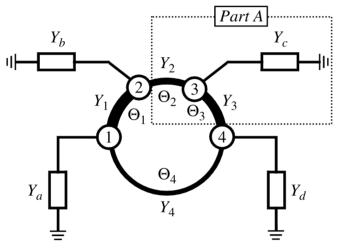
\includegraphics[width=0.5\textwidth]{../assets/review/ring_hybrid.pdf}
			\caption*{
				Fig. A 4-port asymmetric ring hybrid. Here the arc length between ports are $\Theta_1 = \Theta_2 = \Theta_3 = \lambda / 4$ and $\Theta_4 = 3 \lambda / 4$ where $\lambda$ is the wavelength. The termination admittances $Y_a$ to $Y_d$ are arbitrary and the characteristic admittances of transmission-line sections are not necessarily the same, such that the scattering parameters can be asymmetric. Source: modified from \cite{Ahn2006}.
			}
		\end{figure}

		On the other hand, symmetric \gls{ris} satisfying $\mathbf{\Theta} = \mathbf{\Theta}^\mathsf{T}$ are often considered in the literature as they can be implemented with simpler circuit components (e.g., capacitors and inductors).
		We have added Section \ref{sc:ris_symmetry} to investigate the impact of \gls{ris} symmetry on the system performance.

		\change{
			Symmetric \gls{ris} satisfying $\mathbf{\Theta} = \mathbf{\Theta}^\mathsf{T}$ are often considered in the literature due to hardware constraints.
			This study aim to investigate the impact of \gls{ris} symmetry on the system performance.
			\begin{remark}
				All proposed asymmetric \gls{bd}-\gls{ris} designs can be modified for symmetry. In particular,
				\begin{enumerate}[label=(\roman*)]
					\item \emph{\gls{svd}-based (e.g., \eqref{eq:ris_nd_sv_indl}, \eqref{eq:ris_nd_power}, \eqref{eq:ris_nd_rate_max}, \eqref{eq:ris_power}, \eqref{eq:ris_procrustes}):} Those closed-form asymmetric solutions are constructed from the product of singular matrices. If symmetry is required, one can replace the \gls{svd} of $\mathbf{A} = \mathbf{U} \mathbf{\Sigma} \mathbf{V}^\mathsf{H}$ by the Autonne-Takagi factorization of $\frac{\mathbf{A} + \mathbf{A}^\mathsf{T}}{2} = \mathbf{Q} \mathbf{\Sigma} \mathbf{Q}^\mathsf{T}$ \cite{Ikramov2012} and use unitary factor $\mathbf{Q}$ to construct the corresponding $\mathbf{\Theta}$.
					\item \emph{\gls{rcg}-based (e.g., \eqref{eq:shaping_subdiff}, \eqref{eq:gradient_eucl_rate}, \eqref{eq:gradient_eucl_wsr}):} The symmetry constraint is added to the corresponding optimization problems, and one can project the solution to the nearest symmetric point $\mathbf{\Theta} \gets \frac{\mathbf{\Theta} + \mathbf{\Theta}^\mathsf{T}}{2}$ after each iteration.
				\end{enumerate}
			\end{remark}

			\begin{figure}[H]
				\centering
				\subfloat[Power: $2 \times N_\mathrm{S} \times 2$]{
					\resizebox{!}{5cm}{
						% This file was created by matlab2tikz.
%
%The latest updates can be retrieved from
%  http://www.mathworks.com/matlabcentral/fileexchange/22022-matlab2tikz-matlab2tikz
%where you can also make suggestions and rate matlab2tikz.
%
\definecolor{mycolor1}{rgb}{0.00000,0.44706,0.74118}%
\definecolor{mycolor2}{rgb}{0.85098,0.32549,0.09804}%
%
\begin{tikzpicture}

\begin{axis}[%
width=9.509cm,
height=7.5cm,
at={(0cm,0cm)},
scale only axis,
xmin=1,
xmax=7,
xtick={1,2,3,4,5,6,7},
xticklabels={{$2^0$},{$2^1$},{$2^2$},{$2^3$},{$2^4$},{$2^5$},{$2^6$}},
% xlabel style={font=\color{white!15!black}},
xlabel={RIS Group Size},
ymin=0,
ymax=9e-07,
% ylabel style={font=\color{white!15!black}},
ylabel={Channel Power [W]},
axis background/.style={fill=white},
xmajorgrids,
ymajorgrids,
legend style={at={(0.03,0.97)}, anchor=north west, legend cell align=left, align=left, draw=white!15!black}
]
\addplot [color=mycolor1, line width=2.0pt, mark=o, mark options={solid, mycolor1}]
  table[row sep=crcr]{%
1	3.07226159314351e-08\\
2	4.11492399332381e-08\\
3	4.88148530601955e-08\\
4	5.26094766034717e-08\\
5	5.43186358023285e-08\\
};
\addlegendentry{Asymmetric: $N_\mathrm{S} = 16$}

\addplot [color=mycolor1, dashed, line width=2.0pt, mark=o, mark options={solid, mycolor1}]
  table[row sep=crcr]{%
1	3.07226159314351e-08\\
2	2.48110921829919e-08\\
3	2.09999716084868e-08\\
4	1.85392359072275e-08\\
5	1.69392170352418e-08\\
};
\addlegendentry{Enforced: $N_\mathrm{S} = 16$}

\addplot [color=mycolor1, dotted, line width=2.0pt, mark=o, mark options={solid, mycolor1}]
  table[row sep=crcr]{%
1	2.18823167401622e-08\\
2	2.58667252589526e-08\\
3	3.6393122841988e-08\\
4	4.41807731672663e-08\\
5	4.8483723780213e-08\\
};
\addlegendentry{Legacy: $N_\mathrm{S} = 16$}

\addplot [color=mycolor1, dashdotted, line width=2.0pt, mark=o, mark options={solid, mycolor1}]
  table[row sep=crcr]{%
1	3.07226159314351e-08\\
2	3.78824565046636e-08\\
3	4.6008649901077e-08\\
4	5.13929112888468e-08\\
5	5.39731769119744e-08\\
};
\addlegendentry{Takagi: $N_\mathrm{S} = 16$}

\addplot [color=mycolor2, line width=2.0pt, mark=+, mark options={solid, mycolor2}]
  table[row sep=crcr]{%
1	3.73674394477017e-07\\
2	5.420346500246e-07\\
3	6.85389992643681e-07\\
4	7.6227451113248e-07\\
5	8.0069480829595e-07\\
6	8.18206267524393e-07\\
7	8.25088677505729e-07\\
};
\addlegendentry{Asymmetric: $N_\mathrm{S} = 64$}

\addplot [color=mycolor2, dashed, line width=2.0pt, mark=+, mark options={solid, mycolor2}]
  table[row sep=crcr]{%
1	3.73674394477017e-07\\
2	3.06957520044884e-07\\
3	2.68618316241873e-07\\
4	2.45748953801729e-07\\
5	2.27807576071471e-07\\
6	2.22821968007804e-07\\
7	2.16970499497674e-07\\
};
\addlegendentry{Enforced: $N_\mathrm{S} = 64$}

\addplot [color=mycolor2, dotted, line width=2.0pt, mark=+, mark options={solid, mycolor2}]
  table[row sep=crcr]{%
1	3.02768340133104e-07\\
2	3.67874038919462e-07\\
3	5.47929160259681e-07\\
4	6.80081694767098e-07\\
5	7.48298918253076e-07\\
6	7.85561233493806e-07\\
7	8.04051669342744e-07\\
};
\addlegendentry{Legacy: $N_\mathrm{S} = 64$}

\addplot [color=mycolor2, dashdotted, line width=2.0pt, mark=+, mark options={solid, mycolor2}]
  table[row sep=crcr]{%
1	3.73674394477017e-07\\
2	4.73667276858297e-07\\
3	6.21291346950978e-07\\
4	7.28822615730252e-07\\
5	7.83509460162992e-07\\
6	8.10199796739281e-07\\
7	8.22445224822532e-07\\
};
\addlegendentry{Takagi: $N_\mathrm{S} = 64$}

\end{axis}
\end{tikzpicture}%

					}
				}
				\subfloat[Rate: $4 \times N_\mathrm{S} \times 4$]{
					\resizebox{!}{5cm}{
						% This file was created by matlab2tikz.
%
%The latest updates can be retrieved from
%  http://www.mathworks.com/matlabcentral/fileexchange/22022-matlab2tikz-matlab2tikz
%where you can also make suggestions and rate matlab2tikz.
%
\definecolor{mycolor1}{rgb}{0.00000,0.44706,0.74118}%
\definecolor{mycolor2}{rgb}{0.85098,0.32549,0.09804}%
%
\begin{tikzpicture}

\begin{axis}[%
width=11.411cm,
height=9cm,
at={(0cm,0cm)},
scale only axis,
xmin=-20,
xmax=20,
xlabel style={font=\color{white!15!black}},
xlabel={Transmit Power [dB]},
ymin=0,
ymax=60,
ylabel style={font=\color{white!15!black}},
ylabel={Achievable Rate [bit/s/Hz]},
axis background/.style={fill=white},
xmajorgrids,
ymajorgrids,
legend style={at={(0.03,0.97)}, anchor=north west, legend cell align=left, align=left, draw=white!15!black}
]
\addplot [color=black, line width=2.0pt]
  table[row sep=crcr]{%
-20	0.869712506220171\\
-15	2.11804892861715\\
-10	4.32580899488593\\
-5	7.87508759965494\\
0	12.6780205038048\\
5	18.1780871974283\\
10	24.328728256457\\
15	30.8030513368595\\
20	37.3917434238629\\
};
\addlegendentry{No RIS}

\addplot [color=mycolor1, line width=2.0pt, mark=o, mark options={solid, mycolor1}]
  table[row sep=crcr]{%
-20	1.05029082922333\\
-15	2.47337886006358\\
-10	4.92048529343925\\
-5	8.90477411631522\\
0	13.9570874291404\\
5	19.8957463831554\\
10	26.2933401587038\\
15	32.8565936354346\\
20	39.4746708507294\\
};
\addlegendentry{Asymmetric BD: $N_\mathrm{S} = 16$}

\addplot [color=mycolor1, dashed, line width=2.0pt, mark=o, mark options={solid, mycolor1}]
  table[row sep=crcr]{%
-20	0.970760076661331\\
-15	2.3188320234014\\
-10	4.64280739162619\\
-5	8.41835694674129\\
0	13.3604486433245\\
5	19.094165557721\\
10	25.4186344249109\\
15	31.9565133951396\\
20	38.5663724097166\\
};
\addlegendentry{Symmetric-Enforced BD: $N_\mathrm{S} = 16$}

\addplot [color=mycolor1, dotted, line width=2.0pt, mark=o, mark options={solid, mycolor1}]
  table[row sep=crcr]{%
-20	0.97597456292552\\
-15	2.30584921620253\\
-10	4.62292261488193\\
-5	8.33348997224921\\
0	13.3557952177725\\
5	18.9906847997489\\
10	25.437800763079\\
15	31.9385728892858\\
20	38.5311499513319\\
};
\addlegendentry{Symmetric-Projected BD: $N_\mathrm{S} = 16$}

\addplot [color=mycolor2, line width=2.0pt, mark=+, mark options={solid, mycolor2}]
  table[row sep=crcr]{%
-20	3.77847987240857\\
-15	6.50928071370314\\
-10	12.1387730745713\\
-5	18.5875271015713\\
0	24.3077905361749\\
5	33.2971078250378\\
10	39.928680684664\\
15	46.5685472744417\\
20	53.211140381742\\
};
\addlegendentry{Asymmetric BD: $N_\mathrm{S} = 256$}

\addplot [color=mycolor2, dashed, line width=2.0pt, mark=+, mark options={solid, mycolor2}]
  table[row sep=crcr]{%
-20	2.34847395704067\\
-15	4.62061866587552\\
-10	8.87596224335232\\
-5	14.477655849128\\
0	20.072194318481\\
5	28.1693217002636\\
10	34.7805310048903\\
15	41.4138537995477\\
20	48.0542910369292\\
};
\addlegendentry{Symmetric-Enforced BD: $N_\mathrm{S} = 256$}

\addplot [color=mycolor2, dotted, line width=2.0pt, mark=+, mark options={solid, mycolor2}]
  table[row sep=crcr]{%
-20	2.56771808601858\\
-15	4.62163031351707\\
-10	9.02266665728213\\
-5	15.8352879313011\\
0	20.2736387755067\\
5	29.3911431192357\\
10	35.1742881633618\\
15	43.1166685548033\\
20	49.7257139129898\\
};
\addlegendentry{Symmetric-Projected BD: $N_\mathrm{S} = 256$}

\end{axis}
\end{tikzpicture}%
					}
				}
				\caption*{
					Fig. Impact of \gls{ris} symmetry on the power gain and achievable rate of \gls{mimo} point-to-point channel.
				}
			\end{figure}

			Figs. \ref{fg:pc_power_symmetry} and \ref{fg:pc_rate_symmetry} compare the power gain and achievable rate of \gls{mimo} point-to-point channel under asymmetric and various symmetric \gls{ris} configurations.
			Here, `Asymmetric' refers to the benchmark solution by \eqref{eq:ris_power} or \eqref{eq:gradient_eucl_rate}, `Enforced' refers to enforcing symmetry on `Asymmetric', `Legacy' refers to a straightforward extension of the \gls{siso} \gls{snr}-optimal solution \cite[(6)]{Santamaria2023}, `Takagi' refers to the modification \ref{it:takagi}, and `Projection' refers to the modification \ref{it:projection}.
			We observe that the performance gaps between the asymmetric and symmetric \gls{ris} configurations are insignificant and scale with the number of scattering elements.
			The two proposed modifications also outperform other candidates in both problems.
		}
	}

	\comment{
		The geodesic \gls{rcg} method seems promising especially at large group size $L$. Is it possible to extend the design framework to advanced \gls{bd}-\gls{ris} architectures (e.g., multi-sector mode)?
	}

	\reply{
		Unfortunately, the geodesic \gls{rcg} method relies on the block unitary property of the \gls{bd}-\gls{ris} scattering matrix and is not directly applicable to multi-sector mode \gls{bd}-\gls{ris} where the constraint is relaxed to $\sum_{s=1}^S \mathbf{\Theta}_{g,s}^\mathsf{H} \mathbf{\Theta}_{g,s} = \mathbf{I}, \ \forall g \in [G]$ with $S > 1$ sectors.
	}

	\comment{
		For fully-connected \gls{bd}-\gls{ris}, the authors mentioned in the result section that power gain-optimal scattering matrix is also rate-optimal. Can you provide a proof on this point?
	}

	\reply{
		This is indeed an interesting observation.
		When the direct channel is negligible, the power gain-optimal scattering matrix is obtained in closed form \eqref{eq:ris_nd_power_max} and coincides with the rate-optimal scattering matrix \eqref{eq:ris_nd_rate_max} in the newly added Corollary \ref{co:nd_capacity_snr_general}.
		When the direct channel is significant, the observation still holds, yet unfortunately we do not have a formal proof due to the non-trivial structure of both solutions.
		The following context has been added to the manuscript to clarify this point.

		\change{
			Corollary \ref{co:nd_capacity_snr_general} also suggests that the power- and rate-optimal scattering matrices \eqref{eq:ris_nd_power_max} and \eqref{eq:ris_nd_rate_max} coincide with each other when the direct channel is negligible and the \gls{bd}-\gls{ris} is fully-connected.
			When either condition is not satisfied, active and passive beamforming are coupled and the rate-optimal solution involves alternating optimization.
			However, the power-optimal \gls{ris} still provides for a low-complexity decoupled solution.
			The details will be discussed in Section~\ref{sc:rate}.
		}
	}

	\comment{
		The authors refer to \cite{Li2024} for estimating forward and backward channels individually. However, it can be challenging to implement those in real time without RF chains at the \gls{ris}. The impact of imperfect \gls{csi} on the achievable rates may also be studied.
	}

	\reply{
		We agree with the reviewer that the estimation of individual forward and backward channels may be challenging in practice.
		Section \ref{sc:estimation_error} has been added to investigate the impact of imperfect \gls{csi} on the proposed beamforming designs.

		\change{
			\begin{figure}[H]
				\centering
				\resizebox{!}{5cm}{
					% This file was created by matlab2tikz.
%
%The latest updates can be retrieved from
%  http://www.mathworks.com/matlabcentral/fileexchange/22022-matlab2tikz-matlab2tikz
%where you can also make suggestions and rate matlab2tikz.
%
\definecolor{mycolor1}{rgb}{0.00000,0.44706,0.74118}%
\definecolor{mycolor2}{rgb}{0.85098,0.32549,0.09804}%
\definecolor{mycolor3}{rgb}{0.92941,0.69412,0.12549}%
%
\begin{tikzpicture}

\begin{axis}[%
width=9.509cm,
height=7.5cm,
at={(0cm,0cm)},
scale only axis,
xmin=2,
xmax=8,
xlabel style={font=\color{white!15!black}},
xlabel={Number of Transceiver Pairs},
ymin=19.6783408306497,
ymax=31.2584285152524,
ylabel style={font=\color{white!15!black}},
ylabel={Weighted Sum-Rate [bit/s/Hz]},
axis background/.style={fill=white},
xmajorgrids,
ymajorgrids,
legend style={at={(0.03,0.97)}, anchor=north west, legend cell align=left, align=left, draw=white!15!black}
]
\addplot [color=black, line width=2.0pt]
  table[row sep=crcr]{%
2	20.0580414537675\\
3	23.1494203806682\\
4	23.8131916321643\\
5	24.1397335191184\\
6	24.5460196372092\\
7	24.6755028086911\\
8	25.1074670516212\\
};
\addlegendentry{No RIS}

\addplot [color=mycolor1, line width=2.0pt, mark=o, mark options={solid, mycolor1}]
  table[row sep=crcr]{%
2	21.4573948816656\\
3	27.1930653739343\\
4	28.1831089641829\\
5	29.0745868983109\\
6	30.0024676892427\\
7	30.2447444067533\\
8	30.4953140968756\\
};
\addlegendentry{D: $\epsilon = 0.01$}

\addplot [color=mycolor1, dashed, line width=2.0pt, mark=o, mark options={solid, mycolor1}]
  table[row sep=crcr]{%
2	21.9522206635974\\
3	27.9972659014569\\
4	29.1774660072937\\
5	29.8976401507066\\
6	31.2492907400021\\
7	31.0061272412754\\
8	31.2584285152524\\
};
\addlegendentry{BD: $\epsilon = 0.01$}

\addplot [color=mycolor2, line width=2.0pt, mark=+, mark options={solid, mycolor2}]
  table[row sep=crcr]{%
2	21.2137573609231\\
3	26.7691088305489\\
4	27.3922498353221\\
5	28.4987705276947\\
6	28.9805338770942\\
7	29.0123559485939\\
8	29.3028996599066\\
};
\addlegendentry{D: $\epsilon = 0.1$}

\addplot [color=mycolor2, dashed, line width=2.0pt, mark=+, mark options={solid, mycolor2}]
  table[row sep=crcr]{%
2	21.8689236337818\\
3	27.6438667486293\\
4	28.3756628372712\\
5	29.1140292282237\\
6	30.2747006387336\\
7	30.0460875923069\\
8	30.0745412492538\\
};
\addlegendentry{BD: $\epsilon = 0.1$}

\addplot [color=mycolor3, line width=2.0pt, mark=square, mark options={solid, mycolor3}]
  table[row sep=crcr]{%
2	19.6783408306497\\
3	23.5834177542131\\
4	23.4786045133054\\
5	23.9910896622471\\
6	24.3263551713459\\
7	24.3223986465523\\
8	24.2891980094395\\
};
\addlegendentry{D: $\epsilon = 0.5$}

\addplot [color=mycolor3, dashed, line width=2.0pt, mark=square, mark options={solid, mycolor3}]
  table[row sep=crcr]{%
2	20.4883438363461\\
3	23.5557350734111\\
4	23.4446441145768\\
5	23.986245619365\\
6	24.5703590360021\\
7	24.3047930713767\\
8	24.3803426979632\\
};
\addlegendentry{BD: $\epsilon = 0.5$}

\end{axis}
\end{tikzpicture}%
				}
				\caption*{
					Fig. Impact of channel estimation error and transceiver pairs on the weighted sum-rate of $(2 \times 64 \times 2)^K$ \gls{mimo} interference channel with $P = \qty{20}{dB}$ and $N_\mathrm{E} = 2$.
				}
			\end{figure}

			Fig.~\ref{fg:ic_wsr_pair} shows the average \gls{wsr} versus the backward/forward channel estimation error and the number of transceiver pairs.
			Specifically, the active and passive beamformers are designed by Section \ref{sc:rate_ao} over the estimated backward and forward channels
			\begin{equation*}
				\hat{\mathbf{H}}_{\mathrm{B/F}}^{(k)} = \mathbf{H}_{\mathrm{B/F}}^{(k)} + \tilde{\mathbf{H}}_{\mathrm{B/F}}^{(k)}, \quad \forall k,
			\end{equation*}
			where the error follows $\mathrm{vec}(\tilde{\mathbf{H}}_{\mathrm{B/F}}^{(k)}) \sim \mathcal{N}_\mathbb{C}(\mathbf{0}, \epsilon \Lambda_\mathrm{B} \Lambda_\mathrm{F}\mathbf{I})$.
			The \gls{wsr} is evaluated using the true channels.
			We observe that the proposed joint beamforming design in Section \ref{sc:wsr_ao} is reasonably robust to channel estimation error and thus viable for practical implementation.
			On the other hand, introducing a \gls{ris} to \gls{ic} systems is helpful to mitigate the rate saturation effect as $K$ increases.
			In the saturated regime ($K \ge 4$), \gls{bd}-\gls{ris} provides a much larger \gls{wsr} than \gls{d}-\gls{ris} thanks to its superior shaping capability in aligning the interference subspaces.
			These results provide valuable insights for practical \gls{ris} design in dense connection scenarios, where proper \gls{bd} configurations can significantly enhance the network capacity.
		}
	}

	\comment{
		Some sentences are confusing to me and the presentation can be improved. For example, ``a group-wise geodesic \gls{rcg} method that operates directly on the Stiefel manifold''. Please elaborate more on this.
	}

	\reply{
		Thank you for the feedback. The manuscript has been carefully restructured and proofread for improved clarity and readability.
	}

\end{reviewer}


\begin{reviewer}
	\summary{
		This paper analyzes the channel shaping of a \gls{p2p} \gls{mimo} system, assisted by passive diagonal and/or non-diagonal \glspl{ris} to enhance power and rate gains. Overall, the topic is timely and interesting. Using \gls{ao}, a local optimal solution of the rate maximization for the \gls{bd}-\gls{ris}-assisted \gls{mimo} \gls{p2p} system is obtained. It is shown that \gls{bd}-\gls{ris} improve the achievable rate. To the best of my knowledge, the analysis is solid. However, there are some suggestions for improving the paper further.
	}

	\comment{
		The results for the \gls{p2p} system are insightful. However, a \gls{p2p} system is not typically considered a practical system. It is challenging to extend the results to a system with interfering signals, where the goal is not only to enhance the channel gain of the desired links but also simultaneously to reduce the channel gain of the interfering links. It is more interesting to investigate the rate region of $K$-user \glspl{ic}. It is expected that the authors provide an analysis of the (max-min and sum) rate maximization of multi-user \gls{mimo} systems, assisted by \gls{bd}-\glspl{ris}.
	}

	\reply{
		We appreciate the reviewer's positive feedback and insightful suggestion.
		Interference management by \gls{ris} in multi-user \gls{mimo} systems is indeed an interesting topic.
		In the revised manuscript, we have extended the joint beamforming design to a $K$-user \gls{mimo} \gls{ic} system and provided a comprehensive study on \gls{wsr} maximization problem.
		Please refer to Sections \ref{sc:mimo_ic}, \ref{sc:wsr}, and \ref{sc:simulation_wsr} for the model, optimization, and simulation results.

		\change{
			We also consider a \gls{bd}-\gls{ris} aided \gls{mimo} interference channel of $K$ transceiver pairs where each transmitter and receiver has $N_\mathrm{T}$ and $N_\mathrm{R}$ antennas, respectively, and the \gls{bd}-\gls{ris} has $N_\mathrm{S}$ scattering elements.
			This configuration is denoted as $(N_\mathrm{T} \times N_\mathrm{S} \times N_\mathrm{R})^K$.
			Let $\mathbf{H}_\mathrm{D}^{(kj)} \in \mathbb{C}^{N_\mathrm{R} \times N_\mathrm{T}}$, $\mathbf{H}_\mathrm{B}^{(k)} \in \mathbb{C}^{N_\mathrm{R} \times N_\mathrm{S}}$, $\mathbf{H}_\mathrm{F}^{(j)} \in \mathbb{C}^{N_\mathrm{S} \times N_\mathrm{T}}$ denote the direct channel from transmitter $j$ to receiver $k$, the backward channel of receiver $k$, and the forward channel of transmitter $j$, respectively, where $(j,k) \in [K]^2$.
			Assume all transmitter-\gls{ris}-receiver paths share the same \gls{bd}-\gls{ris} scattering matrix $\mathbf{\Theta}$.
			The equivalent channel from transmitter $j$ to receiver $k$ is
			\begin{equation*}
				\mathbf{H}^{(kj)} = \mathbf{H}_\mathrm{D}^{(kj)} + \mathbf{H}_\mathrm{B}^{(k)} \mathbf{\Theta} \mathbf{H}_\mathrm{F}^{(j)} = \mathbf{H}_\mathrm{D}^{(kj)} + \sum_g \mathbf{H}_{\mathrm{B},g}^{(k)} \mathbf{\Theta}_g \mathbf{H}_{\mathrm{F},g}^{(j)},
			\end{equation*}
			where $\mathbf{H}_{\mathrm{B},g}^{(k)} \in \mathbb{C}^{N_\mathrm{R} \times L}$ and $\mathbf{H}_{\mathrm{F},g}^{(j)} \in \mathbb{C}^{L \times N_\mathrm{T}}$ are associated with \gls{ris} group $g$, corresponding to the $(g{-}1)L{+}1$ to $gL$ columns of $\mathbf{H}_{\mathrm{B},g}^{(k)}$ and rows of $\mathbf{H}_{\mathrm{F},g}^{(j)}$, respectively.
		}

		\change{
			On top of \eqref{eq:channel_interference}, the achievable rate of transmission $k$ is
			\begin{equation*}
				R_k = \log \det \biggl(\mathbf{I} + \mathbf{W}_k {\mathbf{H}^{(kj)\mathsf{H}}} \mathbf{Q}_k^{-1} {\mathbf{H}^{(kj)}} \mathbf{W}_k\biggr),
			\end{equation*}
			where $\mathbf{W}_k$ is the precoder at transmitter $k$ and $\mathbf{Q}_k = \sum_{j \ne k} {\mathbf{H}^{(kj)}} \mathbf{W}_j \mathbf{W}_j^\mathsf{H} {\mathbf{H}^{(kj)\mathsf{H}}} + \eta \mathbf{I}$ is the interference-plus-noise covariance matrix at receiver $k$.
			The \gls{wsr} maximization problem for \gls{bd}-\gls{ris}-aided \gls{mimo} interference channel is formulated as
			\begin{maxi*}
				{\scriptstyle{\mathbf{\Theta}, \{\mathbf{W}_k\}_{k \in [K]}}}{\sum_{k=1}^K \rho_k R_k}{}{}
				\addConstraint{\mathbf{\Theta}_g^\mathsf{H} \mathbf{\Theta}_g=\mathbf{I}, \quad \forall g}{}{}
				\addConstraint{\lVert \mathbf{W}_k \rVert _\mathrm{F}^2 \le P_k. \quad \forall k}{}{}
			\end{maxi*}
			where $\rho_k \ge 0$ is the weight associated with transmission $k$.
			This non-convex problem can be solved by extending both solutions covered in Section \ref{sc:rate} as detailed below.
		}

		\change{
				On top of \eqref{eq:channel_interference}, the achievable rate of transmission $k$ is
				\begin{equation*}
					R_k = \log \det \biggl(\mathbf{I} + \mathbf{W}_k {\mathbf{H}^{(kj)\mathsf{H}}} \mathbf{Q}_k^{-1} {\mathbf{H}^{(kj)}} \mathbf{W}_k\biggr),
				\end{equation*}
				where $\mathbf{W}_k$ is the precoder at transmitter $k$ and $\mathbf{Q}_k = \sum_{j \ne k} {\mathbf{H}^{(kj)}} \mathbf{W}_j \mathbf{W}_j^\mathsf{H} {\mathbf{H}^{(kj)\mathsf{H}}} + \eta \mathbf{I}$ is the interference-plus-noise covariance matrix at receiver $k$.
				The \gls{wsr} maximization problem for \gls{bd}-\gls{ris}-aided \gls{mimo} interference channel is formulated as
				\begin{maxi!}
					{\scriptstyle{\mathbf{\Theta}, \{\mathbf{W}_k\}_{k \in [K]}}}{\sum_{k=1}^K \rho_k R_k}{}{}
					\addConstraint{\mathbf{\Theta}_g^\mathsf{H} \mathbf{\Theta}_g=\mathbf{I}, \quad \forall g}{}{}
					\addConstraint{\lVert \mathbf{W}_k \rVert _\mathrm{F}^2 \le P_k. \quad \forall k}{}{}
				\end{maxi!}
				where $\rho_k \ge 0$ is the weight associated with transmission $k$.
				This non-convex problem can be solved by extending both solutions covered in Section \ref{sc:rate} as detailed below.

				\begin{subsubsection}{Alternating Optimization}
					This approach updates $\mathbf{\Theta}$ and $\{\mathbf{W}_k\}_{k \in [K]}$ iteratively until convergence.
					For a given precoder set, the passive beamforming subproblem is
					\begin{maxi!}
						{\scriptstyle{\mathbf{\Theta}}}{\sum_{k=1}^K \rho_k R_k}{}{}
						\addConstraint{\mathbf{\Theta}_g^\mathsf{H} \mathbf{\Theta}_g=\mathbf{I}, \quad \forall g,}{}{}
					\end{maxi!}
					which can be solved optimally by Algorithm \ref{ag:rcg} with the partial derivative given in Lemma \ref{lm:wsr}.

					\setcounter{lemma}{1}
					\begin{lemma}
						The partial derivative of \eqref{ob:wsr_ris} with respect to \gls{bd}-\gls{ris} block $g$ is
						\begin{equation*}
							\begin{split}
								\frac{\partial \rho_k R_k}{\partial \mathbf{\Theta}_g^*} = \sum_{k=1}^K & \rho_k {\mathbf{H}^{(k)\mathsf{H}}_{\mathrm{B},g}} \mathbf{Q}_k^{-1} {\mathbf{H}^{(kk)}} \mathbf{W}_k \mathbf{E}_k \mathbf{W}_k^\mathsf{H} \\
								& \times \bigl({\mathbf{H}_{\mathrm{F},g}^{(k)\mathsf{H}}} - {\mathbf{H}^{(kk)\mathsf{H}}} \mathbf{Q}_k^{-1} \sum_{j \ne k} {\mathbf{H}^{(kj)}} \mathbf{W}_j \mathbf{W}_j^\mathsf{H} {\mathbf{H}^{(j)\mathsf{H}}_{\mathrm{F},g}}\bigr),
							\end{split}
						\end{equation*}
						where $\mathbf{E}_k = \bigl(\mathbf{I} + {\mathbf{W}_k^\mathsf{H}} {\mathbf{H}^{(kk)\mathsf{H}}} \mathbf{Q}_k {\mathbf{H}^{(kk)}} \mathbf{W}_k\bigr)^{-1}$ is the error matrix of receiver $k$.
					\end{lemma}

					\begin{proof}
						Please refer to Appendix~\ref{ap:wsr}.
					\end{proof}

					For a given $\mathbf{\Theta}$, problem \eqref{op:wsr} reduces to conventional precoding design for interference channel.
					A closed-form iterative solution based on mutual information-\gls{mmse} relationship has been proposed in \cite{Shin2012,Negro2010} and we summarize the steps as follows.
					At iteration $r$, the \gls{mmse} combiner at receiver $k$ is
					\begin{equation*}
						\begin{split}
							\mathbf{G}_k^{(r)} &= {\mathbf{W}_k^{(r-1)\mathsf{H}}} {\mathbf{H}^{(kk)\mathsf{H}}} \\
							& \quad \times \bigl(\mathbf{Q}_k^{(r-1)} + {\mathbf{H}^{(kk)}} \mathbf{W}_k^{(r-1)} {\mathbf{W}_k^{(r-1)\mathsf{H}}} {\mathbf{H}^{(kk)\mathsf{H}}}\bigr)^{-1},
						\end{split}
					\end{equation*}
					the corresponding error matrix is
					\begin{equation*}
						\mathbf{E}_k^{(r)} = \bigl(\mathbf{I} + {\mathbf{W}_k^{(r-1)\mathsf{H}}} {\mathbf{H}^{(kk)\mathsf{H}}} \mathbf{Q}_k^{(r-1)} {\mathbf{H}^{(kk)}} \mathbf{W}_k^{(r-1)}\bigr)^{-1},
					\end{equation*}
					and the optimal precoder at transmitter $k$ is given by
					\begin{equation*}
						\begin{split}
							\mathbf{W}_k^{(r)} & = \Bigl(\sum_{j=1}^K {\mathbf{H}^{(jk)\mathsf{H}}} {\mathbf{G}_j^{(r)\mathsf{H}}} \mathbf{\Omega}_k^{(r)} \mathbf{G}_j^{(r)} \mathbf{H}^{(jk)} + \lambda_k^{(r)} \mathbf{I} \Bigr)^{-1} \\
							& \quad \times {\mathbf{H}^{(kk)\mathsf{H}}} {\mathbf{G}_j^{(r)\mathsf{H}}} \mathbf{\Omega}_k^{(r)},
						\end{split}
					\end{equation*}
					where $\mathbf{\Omega}_k^{(r)} = \rho_k {\mathbf{E}_k^{(r)-1}}$ is the mean-square error weight and $\lambda_k^{(r)}$ is the Lagrange multiplier retrievable by bisection \cite{Shin2012} or in closed form \cite{Negro2010}
					\begin{equation*}
						\lambda_k^{(r)} = \frac{\mathrm{tr}\bigl(\eta \mathbf{\Omega}_k^{(r)} \mathbf{G}_k^{(r)}{\mathbf{G}_k^{(r)\mathsf{H}}} + \sum_{j=1}^K (\mathbf{Z}_{kj}^{(r)} - \mathbf{Z}_{jk}^{(r)}) \bigr)}{P_k},
						% \lambda_k^{(r)} = \frac{\mathrm{tr}\bigl(\eta \mathbf{\Omega}_k^{(r)} \mathbf{G}_k^{(r)}{\mathbf{G}_k^{(r)\mathsf{H}}} + \sum_j \mathbf{\Omega}_k^{(r)}\mathbf{T}_{kj}^{(r)} {\mathbf{T}_{kj}^{(r)\mathsf{H}}} - \mathbf{\Omega}_j^{(r)}\mathbf{T}_{jk}^{(r)} {\mathbf{T}_{jk}^{(r)\mathsf{H}}} \bigr)}{P_k},
					\end{equation*}
					where $\mathbf{Z}_{kj}^{(r)} = \mathbf{\Omega}_k^{(r)}\mathbf{T}_{kj}^{(r)} {\mathbf{T}_{kj}^{(r)\mathsf{H}}}$ and $\mathbf{T}_{kj}^{(r)} = \mathbf{G}_k^{(r)} {\mathbf{H}^{(kj)}} \mathbf{W}_j^{(r)}$.

					The computational complexity of solving subproblem \eqref{op:wsr_ris} by geodesic \gls{rcg} is $\mathcal{O}\bigl(I_\text{RCG} G (N_\mathrm{T} d^2 + N_\mathrm{T}^2 d + N_\mathrm{T}^2 N_\mathrm{R} + N_\mathrm{T} N_\mathrm{R}^2 + K (N_\mathrm{T} N_\mathrm{R} d + N_\mathrm{T} N_\mathrm{R} L) + I_\text{BLS}L^3)\bigr)$.
					That is, $\mathcal{O}_\mathrm{D}\bigl(N_\mathrm{S}\bigr)$ for \gls{d}-\gls{ris} and $\mathcal{O}_\mathrm{BD}\bigl(N_\mathrm{S}^3\bigr)$ for fully-connected \gls{bd}-\gls{ris}.
				\end{subsubsection}

				\begin{subsubsection}{Low-Complexity Solution}
					Similar to Section \ref{sc:rate_lc}, we suboptimally decouple the beamforming design by first shape the channel by \gls{ris} for minimum leakage interference and then optimize the active beamforming.
					The leakage interference minimization problem is formulated as
					\begin{mini*}
						{\scriptstyle{\mathbf{\Theta}}}{I = \sum_{k=1}^K \sum_{j \ne k} \left\lVert {\mathbf{H}}^{(kj)}_\mathrm{D} + {\mathbf{H}}^{(k)}_\mathrm{B} \mathbf{\Theta} {\mathbf{H}}^{(j)}_\mathrm{F} \right\rVert _{\mathrm{F}}^2}{}{}
						\addConstraint{\mathbf{\Theta}_g^\mathsf{H} \mathbf{\Theta}_g=\mathbf{I}, \quad \forall g,}{}{}
					\end{mini*}
					which can be solved iteratively in closed form.

					\begin{proposition}
						Starting from any feasible $\mathbf{\Theta}^{(0)}$, the sequence
						\begin{equation*}
							\mathbf{\Theta}_g^{(r+1)} = \mathbf{U}_g^{(r)} \mathbf{V}_g^{(r)}, \quad \forall g
						\end{equation*}
						monotonically decreases the objective function \eqref{ob:interference},
						% converges to a stationary point of \eqref{op:interference},
						where $\mathbf{U}_g^{(r)}$ and $\mathbf{V}_g^{(r)}$ are any left and right singular matrices of
						\begin{equation*}
							\mathbf{M}_g^{(r)} = \sum_{k=1}^K \sum_{j \ne k} \bigl(\mathbf{B}_g^{(k)} \mathbf{\Theta}_g^{(r)} \mathbf{H}^{(j)}_{\mathrm{F},g} - {\mathbf{H}^{(k)\mathsf{H}}_{\mathrm{B},g}} {\mathbf{D}^{(kj)(r)}_{g}}\bigr) {\mathbf{H}^{(j)\mathsf{H}}_{\mathrm{F},g}},
						\end{equation*}
						where $\mathbf{B}_g^{(k)} = \lambda_1\bigl({\mathbf{H}^{(k)\mathsf{H}}_{\mathrm{B},g}} \mathbf{H}^{(k)}_{\mathrm{B},g}\bigr) \mathbf{I} - {\mathbf{H}^{(k)\mathsf{H}}_{\mathrm{B},g}} \mathbf{H}^{(k)}_{\mathrm{B},g}$ and ${\mathbf{D}^{(kj)(r)}_{g}} = \mathbf{H}^{(kj)}_\mathrm{D} + \sum_{g'<g} {\mathbf{H}_{\mathrm{B},g'}^{(k)\mathsf{H}}} \mathbf{\Theta}_{g'}^{(r+1)} \mathbf{H}_{\mathrm{F},g'}^{(k)} + \sum_{g'>g} {\mathbf{H}_{\mathrm{B},g'}^{(k)\mathsf{H}}} \mathbf{\Theta}_{g'}^{(r)} \mathbf{H}_{\mathrm{F},g'}^{(k)}.$
						Besides, when \eqref{eq:auxiliary_interference} converges, \eqref{eq:ris_interference} leads to a convergence of the objective function \eqref{ob:interference} towards a stationary point.
					\end{proposition}
					\begin{proof}
						Please refer to Appendix~\ref{ap:interference}.
					\end{proof}
					Once the channel is shaped by \eqref{eq:ris_interference}, the active beamforming is retrieved iteratively by \eqref{eq:precoder_wsr}.
					This two-stage solution avoids outer iterations and efficiently handles inner iterations.
				\end{subsubsection}
		}

		\change{
			\setcounter{subfigure}{0}
			\begin{figure}[H]
				\centering
				\subfloat[Interference: $(4 \times N_\mathrm{S} \times 4)^5$]{
					\resizebox{!}{5cm}{
						% This file was created by matlab2tikz.
%
%The latest updates can be retrieved from
%  http://www.mathworks.com/matlabcentral/fileexchange/22022-matlab2tikz-matlab2tikz
%where you can also make suggestions and rate matlab2tikz.
%
\definecolor{mycolor1}{rgb}{0.00000,0.44706,0.74118}%
\definecolor{mycolor2}{rgb}{0.85098,0.32549,0.09804}%
\definecolor{mycolor3}{rgb}{0.92941,0.69412,0.12549}%
\definecolor{mycolor4}{rgb}{0.49412,0.18431,0.55686}%
%
\begin{tikzpicture}

\begin{axis}[%
width=7.607cm,
height=6cm,
at={(0cm,0cm)},
scale only axis,
xmin=1,
xmax=9,
xtick={1,2,3,4,5,6,7,8,9},
xticklabels={{$2^0$},{$2^1$},{$2^2$},{$2^3$},{$2^4$},{$2^5$},{$2^6$},{$2^7$},{$2^8$}},
xlabel style={font=\color{white!15!black}},
xlabel={RIS Group Size},
ymin=0.00302,
ymax=0.0032,
ylabel style={font=\color{white!15!black}},
ylabel={Leakage Interference [W]},
axis background/.style={fill=white},
xmajorgrids,
ymajorgrids,
legend style={legend cell align=left, align=left, draw=white!15!black}
]
\addplot [color=black, line width=2.0pt]
  table[row sep=crcr]{%
1	0.00319162741340851\\
2	0.00319162741340851\\
3	0.00319162741340851\\
4	0.00319162741340851\\
5	0.00319162741340851\\
6	0.00319162741340851\\
7	0.00319162741340851\\
8	0.00319162741340851\\
9	0.00319162741340851\\
};
\addlegendentry{No RIS}

\addplot [color=mycolor1, line width=2.0pt]
  table[row sep=crcr]{%
1	0.0031903807511434\\
2	0.00319000858789868\\
3	0.00318948243565719\\
};
\addlegendentry{$N_\mathrm{S} = 4$}

\addplot [color=mycolor2, dashed, line width=2.0pt]
  table[row sep=crcr]{%
1	0.00318715155671877\\
2	0.00318564573776907\\
3	0.00318341720398391\\
4	0.00318164867929578\\
5	0.00318044603427818\\
};
\addlegendentry{$N_\mathrm{S} = 16$}

\addplot [color=mycolor3, dotted, line width=2.0pt]
  table[row sep=crcr]{%
1	0.00317233445297942\\
2	0.00316632375843254\\
3	0.00315884531688785\\
4	0.00315347945673859\\
5	0.0031495565085029\\
6	0.00314727430400366\\
7	0.00314627637231178\\
};
\addlegendentry{$N_\mathrm{S} = 64$}

\addplot [color=mycolor4, dashdotted, line width=2.0pt]
  table[row sep=crcr]{%
1	0.00312584848467527\\
2	0.00310531867736959\\
3	0.003082057965558\\
4	0.00306286314221711\\
5	0.00305050875955848\\
6	0.00304378672802381\\
7	0.00304085124667151\\
8	0.00303957035068273\\
9	0.00303912345954656\\
};
\addlegendentry{$N_\mathrm{S} = 256$}

\end{axis}
\end{tikzpicture}%
					}
				}
				\subfloat[WSR: $(2 \times 128 \times 2)^2, N_\mathrm{E} = 2$]{
					\resizebox{!}{5cm}{
						% This file was created by matlab2tikz.
%
%The latest updates can be retrieved from
%  http://www.mathworks.com/matlabcentral/fileexchange/22022-matlab2tikz-matlab2tikz
%where you can also make suggestions and rate matlab2tikz.
%
\definecolor{mycolor1}{rgb}{0.00000,0.44706,0.74118}%
\definecolor{mycolor2}{rgb}{0.85098,0.32549,0.09804}%
%
\begin{tikzpicture}

\begin{axis}[%
width=9.509cm,
height=7.5cm,
at={(0cm,0cm)},
scale only axis,
xmin=-20,
xmax=20,
xlabel style={font=\color{white!15!black}},
xlabel={Transmit Power [dB]},
ymin=7.45838436661787,
ymax=69.663861702895,
ylabel style={font=\color{white!15!black}},
ylabel={Weighted Sum-Rate [bit/s/Hz]},
axis background/.style={fill=white},
xmajorgrids,
ymajorgrids,
legend style={at={(0.03,0.97)}, anchor=north west, legend cell align=left, align=left, draw=white!15!black}
]
\addplot [color=black, line width=2.0pt]
  table[row sep=crcr]{%
-20	7.45838436661787\\
-15	11.8933730551817\\
-10	17.4724560804708\\
-5	23.9064383662022\\
0	30.2586116005037\\
5	37.1613774242372\\
10	44.0728992293035\\
15	50.6510068145007\\
20	56.7288095434996\\
};
\addlegendentry{No RIS}

\addplot [color=mycolor1, line width=2.0pt, mark=o, mark options={solid, mycolor1}]
  table[row sep=crcr]{%
-20	8.39400963532917\\
-15	13.3693241707656\\
-10	19.6895535941668\\
-5	27.0080392882743\\
0	34.6776701299644\\
5	42.2629739498658\\
10	49.8743740545584\\
15	57.1729163162531\\
20	62.4105345708051\\
};
\addlegendentry{Alternate: $L = 1$}

\addplot [color=mycolor1, dashed, line width=2.0pt, mark=o, mark options={solid, mycolor1}]
  table[row sep=crcr]{%
-20	7.53405688899552\\
-15	12.0015932544605\\
-10	17.7043301086301\\
-5	24.0846008767917\\
0	31.0738414649981\\
5	37.1708989907985\\
10	44.1441874249302\\
15	50.7283594917508\\
20	56.7115817001137\\
};
\addlegendentry{Decouple: $L = 1$}

\addplot [color=mycolor2, line width=2.0pt, mark=+, mark options={solid, mycolor2}]
  table[row sep=crcr]{%
-20	9.37207649536277\\
-15	15.123010131597\\
-10	22.2760921744364\\
-5	30.6280650021185\\
0	39.3257852049283\\
5	47.7716729930312\\
10	55.8623295730896\\
15	63.4276496773933\\
20	69.663861702895\\
};
\addlegendentry{Alternate: $L = 128$}

\addplot [color=mycolor2, dashed, line width=2.0pt, mark=+, mark options={solid, mycolor2}]
  table[row sep=crcr]{%
-20	7.63709721488115\\
-15	12.2494620386778\\
-10	18.1988981705091\\
-5	25.0504864566346\\
0	32.1207531846306\\
5	38.7526348277966\\
10	45.3327562326459\\
15	51.9651427074415\\
20	58.085388651383\\
};
\addlegendentry{Decouple: $L = 128$}

\end{axis}
\end{tikzpicture}%
					}
				}
				\\
				\subfloat[WSR: $(4 \times N_\mathrm{S} \times 4)^5, N_\mathrm{E} = 4$]{
					\resizebox{!}{5cm}{
						% This file was created by matlab2tikz.
%
%The latest updates can be retrieved from
%  http://www.mathworks.com/matlabcentral/fileexchange/22022-matlab2tikz-matlab2tikz
%where you can also make suggestions and rate matlab2tikz.
%
\definecolor{mycolor1}{rgb}{0.00000,0.44706,0.74118}%
\definecolor{mycolor2}{rgb}{0.85098,0.32549,0.09804}%
%
\begin{tikzpicture}

\begin{axis}[%
width=9.509cm,
height=7.5cm,
at={(0cm,0cm)},
scale only axis,
xmin=-20,
xmax=20,
xlabel style={font=\color{white!15!black}},
xlabel={Transmit Power [dB]},
ymin=1.80960235529644,
ymax=51.8736026387268,
ylabel style={font=\color{white!15!black}},
ylabel={Weighted Sum-Rate [bit/s/Hz]},
axis background/.style={fill=white},
xmajorgrids,
ymajorgrids,
legend style={at={(0.03,0.97)}, anchor=north west, legend cell align=left, align=left, draw=white!15!black}
]
\addplot [color=black, line width=2.0pt]
  table[row sep=crcr]{%
-20	1.80960235529644\\
-15	4.11098690111273\\
-10	7.75480768994706\\
-5	12.3629407741576\\
0	17.1024545214966\\
5	23.1625681731557\\
10	26.8707626601197\\
15	32.4613458700836\\
20	37.8123132871494\\
};
\addlegendentry{No RIS}

\addplot [color=mycolor1, line width=2.0pt, mark=o, mark options={solid, mycolor1}]
  table[row sep=crcr]{%
-20	1.84090112841091\\
-15	4.17316547089654\\
-10	7.87627713234468\\
-5	12.5547901376589\\
0	18.1717345117433\\
5	24.4285668007629\\
10	31.1701707083556\\
15	38.1109874738279\\
20	44.7063377254754\\
};
\addlegendentry{D: $N_\mathrm{S} = 16$}

\addplot [color=mycolor1, dashed, line width=2.0pt, mark=o, mark options={solid, mycolor1}]
  table[row sep=crcr]{%
-20	1.88546551946957\\
-15	4.26755277591478\\
-10	8.03513981766996\\
-5	12.7981637199047\\
0	18.4812179327446\\
5	24.8490348256226\\
10	31.7936364203311\\
15	39.0286092135366\\
20	46.8062457763876\\
};
\addlegendentry{BD: $N_\mathrm{S} = 16$}

\addplot [color=mycolor2, line width=2.0pt, mark=+, mark options={solid, mycolor2}]
  table[row sep=crcr]{%
-20	1.98179894898587\\
-15	4.45391293669394\\
-10	8.35205508799969\\
-5	13.3699181438676\\
0	19.3427348063838\\
5	25.9798496564916\\
10	33.1775440661637\\
15	40.9772485437591\\
20	48.9939947810991\\
};
\addlegendentry{D: $N_\mathrm{S} = 64$}

\addplot [color=mycolor2, dashed, line width=2.0pt, mark=+, mark options={solid, mycolor2}]
  table[row sep=crcr]{%
-20	2.24253273733089\\
-15	4.9947328987611\\
-10	9.26935272982558\\
-5	14.7180807744025\\
0	21.0764272566916\\
5	28.3040251152033\\
10	36.0249159599467\\
15	44.0132822374012\\
20	51.8736026387268\\
};
\addlegendentry{BD: $N_\mathrm{S} = 64$}

\end{axis}

\begin{axis}[%
width=12.27cm,
height=9.202cm,
at={(-1.595cm,-1.012cm)},
scale only axis,
xmin=0,
xmax=1,
ymin=0,
ymax=1,
axis line style={draw=none},
ticks=none,
axis x line*=bottom,
axis y line*=left
]
\end{axis}
\end{tikzpicture}%

					}
				}
				\subfloat[WSR: $(N_\mathrm{T} \times 128 \times N_\mathrm{R})^{10}, N_\mathrm{E} = 2$]{
					\resizebox{!}{5cm}{
						% This file was created by matlab2tikz.
%
%The latest updates can be retrieved from
%  http://www.mathworks.com/matlabcentral/fileexchange/22022-matlab2tikz-matlab2tikz
%where you can also make suggestions and rate matlab2tikz.
%
\definecolor{mycolor1}{rgb}{0.00000,0.44706,0.74118}%
\definecolor{mycolor2}{rgb}{0.85098,0.32549,0.09804}%
\definecolor{mycolor3}{rgb}{0.92941,0.69412,0.12549}%
%
\begin{tikzpicture}

\begin{axis}[%
width=9.509cm,
height=7.5cm,
at={(0cm,0cm)},
scale only axis,
xmin=-20,
xmax=20,
xlabel style={font=\color{white!15!black}},
xlabel={Transmit Power [dB]},
ymin=7.83733686074299,
ymax=149.419217962719,
ylabel style={font=\color{white!15!black}},
ylabel={Weighted Sum-Rate [bit/s/Hz]},
axis background/.style={fill=white},
xmajorgrids,
ymajorgrids,
legend style={at={(0.03,0.97)}, anchor=north west, legend cell align=left, align=left, draw=white!15!black}
]
\addplot [color=mycolor1, line width=2.0pt, mark=o, mark options={solid, mycolor1}]
  table[row sep=crcr]{%
-20	7.83948121186516\\
-15	10.1015091609019\\
-10	12.0004233682033\\
-5	14.6380966326283\\
0	17.4628816797072\\
5	20.7218464633297\\
10	24.6545958788906\\
15	28.2726428196513\\
20	31.7315951609709\\
};
\addlegendentry{D: $N_\mathrm{T}=N_\mathrm{R} = 2$}

\addplot [color=mycolor1, dashed, line width=2.0pt, mark=o, mark options={solid, mycolor1}]
  table[row sep=crcr]{%
-20	7.83733686074299\\
-15	10.0193736667404\\
-10	12.9435742408175\\
-5	16.2677883526666\\
0	20.5526114639166\\
5	24.6234221157436\\
10	29.1511157299157\\
15	33.0713533525499\\
20	35.8147739447367\\
};
\addlegendentry{BD: $N_\mathrm{T}=N_\mathrm{R} = 2$}

\addplot [color=mycolor2, line width=2.0pt, mark=+, mark options={solid, mycolor2}]
  table[row sep=crcr]{%
-20	15.1209129283955\\
-15	19.8413816594543\\
-10	25.4981075377296\\
-5	32.7715081751928\\
0	41.198846706205\\
5	48.3131886751132\\
10	55.8086808857495\\
15	62.1787080102253\\
20	68.0551431649622\\
};
\addlegendentry{D: $N_\mathrm{T}=N_\mathrm{R} = 4$}

\addplot [color=mycolor2, dashed, line width=2.0pt, mark=+, mark options={solid, mycolor2}]
  table[row sep=crcr]{%
-20	15.7176086227888\\
-15	21.4102495156061\\
-10	28.5986790440202\\
-5	37.4538565425314\\
0	46.6609659124334\\
5	56.0296672333454\\
10	64.8867309162011\\
15	72.3750621241665\\
20	75.7859933518656\\
};
\addlegendentry{BD: $N_\mathrm{T}=N_\mathrm{R} = 4$}

\addplot [color=mycolor3, line width=2.0pt, mark=square, mark options={solid, mycolor3}]
  table[row sep=crcr]{%
-20	25.7988635393337\\
-15	35.9236746342655\\
-10	49.1052350660732\\
-5	65.0727389847456\\
0	81.7530229815014\\
5	96.0295529130877\\
10	110.587455583348\\
15	124.954201920781\\
20	136.174808834443\\
};
\addlegendentry{D: $N_\mathrm{T}=N_\mathrm{R} = 8$}

\addplot [color=mycolor3, dashed, line width=2.0pt, mark=square, mark options={solid, mycolor3}]
  table[row sep=crcr]{%
-20	26.9797451957892\\
-15	38.1104897727695\\
-10	52.981441121311\\
-5	71.1782472996108\\
0	90.3831761453612\\
5	108.266417508482\\
10	125.160228915665\\
15	139.75853685782\\
20	149.419217962719\\
};
\addlegendentry{BD: $N_\mathrm{T}=N_\mathrm{R} = 8$}

\end{axis}
\end{tikzpicture}%
					}
				}
				\caption*{
					Fig. Average leakage interference and weighted sum-rate versus \gls{ris} and \gls{mimo} interference channel configurations.
					`Alternate' refers to the alternating optimization and `Decouple' refers to the low-complexity design.
					`D' means \gls{d}-\gls{ris} and `BD' refers to fully-connected \gls{bd}-\gls{ris}.
				}
			\end{figure}

			Fig.~\ref{fg:ic_interference_sx} illustrates how \gls{bd}-\gls{ris} helps to reduce the leakage interference by solving problem \eqref{op:interference}.
			In this case, a fully-connected $2^n$-element \gls{bd}-\gls{ris} is almost as good as a $2^{n+2}$-element \gls{d}-\gls{ris} in terms of leakage interference.
			The result also implies that \gls{bd}-\gls{ris} can achieve a higher \gls{dof} than diagonal \gls{ris} in \gls{mimo} interference channel, which generalizes Proposition \ref{pp:dof} and emphasizes the potential of \gls{bd}-\gls{ris} in interference alignment.

			Fig.~\ref{fg:ic_wsr_beamforming} compares the average \gls{wsr} achieved by the optimal and low-complexity beamforming designs in Section \ref{sc:wsr_ao} and \ref{sc:wsr_lc}, respectively.
			Unlike the point-to-point case, the latter is not as effective as the former.
			The reason is that, for $K$ transmissions of different path loss, interference alignment using only a shared passive beamformer is very challenging especially, when the direct channels are dominant.
			On the other hand, using $K$ precoders in the joint beamforming design can reasonably orthogonalize the channels and the \gls{ris} can simply enhance the signal power.
			A narrower performance gap is expected when $N_\mathrm{S}$ increases or \gls{ris} coverage area shrinks.

			Figs.~\ref{fg:ic_wsr_sx} and \ref{fg:ic_wsr_txrx} show the average \gls{wsr} versus the number of scattering elements and transceiving antennas.
			Again, we observe that the rate gain of \gls{bd}-\gls{ris} over \gls{d}-\gls{ris} increases with $N_\mathrm{S}$, $N_\mathrm{T}$, and $N_\mathrm{R}$.
			The reasons have been discussed in the point-to-point case.

			\begin{figure}[H]
				\centering
				\resizebox{!}{5cm}{
					% This file was created by matlab2tikz.
%
%The latest updates can be retrieved from
%  http://www.mathworks.com/matlabcentral/fileexchange/22022-matlab2tikz-matlab2tikz
%where you can also make suggestions and rate matlab2tikz.
%
\definecolor{mycolor1}{rgb}{0.00000,0.44706,0.74118}%
\definecolor{mycolor2}{rgb}{0.85098,0.32549,0.09804}%
\definecolor{mycolor3}{rgb}{0.92941,0.69412,0.12549}%
%
\begin{tikzpicture}

\begin{axis}[%
width=9.509cm,
height=7.5cm,
at={(0cm,0cm)},
scale only axis,
xmin=2,
xmax=8,
xlabel style={font=\color{white!15!black}},
xlabel={Number of Transceiver Pairs},
ymin=19.6783408306497,
ymax=31.2584285152524,
ylabel style={font=\color{white!15!black}},
ylabel={Weighted Sum-Rate [bit/s/Hz]},
axis background/.style={fill=white},
xmajorgrids,
ymajorgrids,
legend style={at={(0.03,0.97)}, anchor=north west, legend cell align=left, align=left, draw=white!15!black}
]
\addplot [color=black, line width=2.0pt]
  table[row sep=crcr]{%
2	20.0580414537675\\
3	23.1494203806682\\
4	23.8131916321643\\
5	24.1397335191184\\
6	24.5460196372092\\
7	24.6755028086911\\
8	25.1074670516212\\
};
\addlegendentry{No RIS}

\addplot [color=mycolor1, line width=2.0pt, mark=o, mark options={solid, mycolor1}]
  table[row sep=crcr]{%
2	21.4573948816656\\
3	27.1930653739343\\
4	28.1831089641829\\
5	29.0745868983109\\
6	30.0024676892427\\
7	30.2447444067533\\
8	30.4953140968756\\
};
\addlegendentry{D: $\epsilon = 0.01$}

\addplot [color=mycolor1, dashed, line width=2.0pt, mark=o, mark options={solid, mycolor1}]
  table[row sep=crcr]{%
2	21.9522206635974\\
3	27.9972659014569\\
4	29.1774660072937\\
5	29.8976401507066\\
6	31.2492907400021\\
7	31.0061272412754\\
8	31.2584285152524\\
};
\addlegendentry{BD: $\epsilon = 0.01$}

\addplot [color=mycolor2, line width=2.0pt, mark=+, mark options={solid, mycolor2}]
  table[row sep=crcr]{%
2	21.2137573609231\\
3	26.7691088305489\\
4	27.3922498353221\\
5	28.4987705276947\\
6	28.9805338770942\\
7	29.0123559485939\\
8	29.3028996599066\\
};
\addlegendentry{D: $\epsilon = 0.1$}

\addplot [color=mycolor2, dashed, line width=2.0pt, mark=+, mark options={solid, mycolor2}]
  table[row sep=crcr]{%
2	21.8689236337818\\
3	27.6438667486293\\
4	28.3756628372712\\
5	29.1140292282237\\
6	30.2747006387336\\
7	30.0460875923069\\
8	30.0745412492538\\
};
\addlegendentry{BD: $\epsilon = 0.1$}

\addplot [color=mycolor3, line width=2.0pt, mark=square, mark options={solid, mycolor3}]
  table[row sep=crcr]{%
2	19.6783408306497\\
3	23.5834177542131\\
4	23.4786045133054\\
5	23.9910896622471\\
6	24.3263551713459\\
7	24.3223986465523\\
8	24.2891980094395\\
};
\addlegendentry{D: $\epsilon = 0.5$}

\addplot [color=mycolor3, dashed, line width=2.0pt, mark=square, mark options={solid, mycolor3}]
  table[row sep=crcr]{%
2	20.4883438363461\\
3	23.5557350734111\\
4	23.4446441145768\\
5	23.986245619365\\
6	24.5703590360021\\
7	24.3047930713767\\
8	24.3803426979632\\
};
\addlegendentry{BD: $\epsilon = 0.5$}

\end{axis}
\end{tikzpicture}%
				}
				\caption*{
					Fig. Impact of channel estimation error and transceiver pairs on the weighted sum-rate of $(2 \times 64 \times 2)^K$ \gls{mimo} interference channel with $P = \qty{20}{dB}$ and $N_\mathrm{E} = 2$.
				}
			\end{figure}

			Fig.~\ref{fg:ic_wsr_pair} shows the average \gls{wsr} versus the backward/forward channel estimation error and the number of transceiver pairs.
			Specifically, the active and passive beamformers are designed by Section \ref{sc:rate_ao} over the estimated backward and forward channels
			\begin{equation*}
				\hat{\mathbf{H}}_{\mathrm{B/F}}^{(k)} = \mathbf{H}_{\mathrm{B/F}}^{(k)} + \tilde{\mathbf{H}}_{\mathrm{B/F}}^{(k)}, \quad \forall k,
			\end{equation*}
			where the error follows $\mathrm{vec}(\tilde{\mathbf{H}}_{\mathrm{B/F}}^{(k)}) \sim \mathcal{N}_\mathbb{C}(\mathbf{0}, \epsilon \Lambda_\mathrm{B} \Lambda_\mathrm{F}\mathbf{I})$.
			The \gls{wsr} is evaluated using the true channels.
			We observe that the proposed joint beamforming design in Section \ref{sc:wsr_ao} is reasonably robust to channel estimation error and thus viable for practical implementation.
			On the other hand, introducing a \gls{ris} to interference channel systems is helpful to mitigate the rate saturation effect as $K$ increases.
			In the saturated regime ($K \ge 4$), \gls{bd}-\gls{ris} provides a much larger \gls{wsr} than \gls{d}-\gls{ris} thanks to its superior shaping capability in aligning the interference subspaces.
			These results provide valuable insights for practical \gls{ris} design in dense connection scenarios, where proper \gls{bd} configurations can significantly enhance the network capacity.
		}
	}

	\comment{
		\gls{bd}-\glspl{ris} provide a greater number of optimization variables but at the expense of increased computational and implementation complexities. While the computational complexities of the proposed solutions are discussed in the paper, a comparison with \gls{d}-\gls{ris} is missing, which should be explicitly addressed in both the introduction and the main body. Additionally, the implementation complexities of \gls{bd}-\glspl{ris}, particularly in comparison to \gls{d}-\gls{ris}, necessitate a more comprehensive analysis. For instance, as highlighted in \cite{Soleymani2024b}, the energy efficiency of a \gls{bd}-\gls{ris} is significantly influenced by the static power consumption of its circuit elements. If the implementation cost of a \gls{bd}-\gls{ris} is substantial, its performance advantages could be considerably reduced.
	}

	\reply{
		We agree with the reviewer that the computational complexities of \gls{d}-\gls{ris} and fully-connected \gls{bd}-\gls{ris} deserve further attention.
		Apart from a summary in the introduction and an explicit analysis in the main body, we have also evaluated the average statistics of the \gls{ao} design for both architectures on the rate maximization problem \eqref{op:rate}.

		On the other hand, the implementation complexities of \gls{bd}-\gls{ris} is indeed a critical issue.
		An initial study has been conducted in \cite{Zhou2023} where the authors demonstrated the superior energy efficiency of \gls{bd}-\gls{ris} compared to both active \gls{ris} and relay systems.
		Our colleagues are currently working on a more comprehensive analysis and the results will be published in a separate paper.

		\change{
			The additional optimization cost of \gls{bd}-\gls{ris} over \gls{d}-\gls{ris} is affordable and the geodesic \gls{rcg} method is efficient on large-scale problems;
		}

		\change{
			That is, $\mathcal{O}_\mathrm{D}\bigl(N_\mathrm{S}\bigr)$ for \gls{d}-\gls{ris} and $\mathcal{O}_\mathrm{BD}\bigl(N_\mathrm{S}^3\bigr)$ for fully-connected \gls{bd}-\gls{ris}.
		}

		\change{
			\begin{table}[H]
				\caption*{Table: Performance of \gls{d}-\gls{ris} and Fully-Connected \gls{bd}-\gls{ris} on \eqref{op:rate}}
				\centering
				\resizebox{\columnwidth}{!}{
					\begin{tabular}{ccccccc}
						\toprule
						\multirow{3}{*}{\gls{ris} type} & \multicolumn{3}{c}{$N_\mathrm{S}=16$} & \multicolumn{3}{c}{$N_\mathrm{S}=256$}                                                               \\ \cmidrule(lr){2-4} \cmidrule(lr){5-7}
														& Objective                             & \begin{tabular}{@{}c@{}}Iterations\\(outer)\end{tabular}                             & Time [s]         & Objective        & \begin{tabular}{@{}c@{}}Iterations\\(outer)\end{tabular} & Time [s] \\ \midrule
						Diagonal                        & $\num{25.33}$                      & 2.06                                  & $\num{2.620e-2}$ & $\num{32.22}$ & 2.92      & 1.277    \\
						Fully-connected BD              & $\num{26.10}$                      & 3.84                                  & $\num{2.719e-2}$ & $\num{36.58}$ & 3.03      & 0.806    \\ \bottomrule
					\end{tabular}
				}
			\end{table}
			Table \ref{tb:complexity_bond} compares the performance of \gls{d}-\gls{ris} and fully-connected \gls{bd}-\gls{ris} on rate maximization problem \eqref{op:rate} using the \gls{ao} design in Section \ref{sc:rate_ao}, where $N_\mathrm{T}=N_\mathrm{R}=4$ and $P=\qty{20}{dB}$.
			The statistics are averaged over \num{100} independent runs.
			The fact that fully-connected \gls{bd}-\gls{ris} provides a higher achievable rate using slightly more outer iterations $I_\text{AO}$ than \gls{d}-\gls{ris} is consistent with our analysis.
			Interestingly, \emph{the former still ends up with shorter elapsed time,} which seems to contradict the complexity analysis that $\mathcal{O}_\mathrm{BD}\bigl(N_\mathrm{S}^3\bigr)$ for fully-connected \gls{bd}-\gls{ris} and $\mathcal{O}_\mathrm{D}\bigl(N_\mathrm{S}\bigr)$ for \gls{d}-\gls{ris}.
			One possible reason is that \gls{bd}-\gls{ris} only involves 1 backtracking line search per iteration while \gls{d}-\gls{ris} requires $N_\mathrm{S}$ times.
			Another reason is that the group-wise update of \gls{d}-\gls{ris} leads to slower convergence of inner iterations.
			These results suggest that optimizing \gls{bd}-\gls{ris} may be less computational intensive than expected.
		}
	}

	\comment{
		The authors considered a passive \gls{ris} architecture. However, another passive configuration, termed \gls{gp}, is discussed in \cite{Fotock2023,Soleymani2024a}. Employing \gls{ao}, the resulting optimization problem to update $\mathbf{\Theta}$ is convex. Comparing the proposed solutions with a globally passive \gls{bd}-\gls{ris} would provide valuable insights into the performance gains obtained by relaxing the (locally) passive assumption. Hence, it is highly recommended to add the \gls{gp} (both \gls{bd} and diagonal) architecture as a benchmark in the numerical results.
	}

	\reply{
		We appreciate the reviewer's suggestion and agree that the \gls{gp} architecture may serve as a canonical benchmark.
		However, the current manuscript already exceeds the page limit and we decided not to overwhelm the readers with too many fancy \gls{ris} configurations.
		An in-depth comparison between \gls{gp} and \gls{bd} architectures holds significant value to the \gls{ris} community and deserves a separate study in the future.
	}

\end{reviewer}


\bibliographystyle{IEEEtran}
\bibliography{supplement}
\end{document}
